\documentclass[a4paper]{article}
\usepackage{array} 
\usepackage{amsmath}
\usepackage{amssymb}
\usepackage{amsthm}
\usepackage{amstext} 
\usepackage{amsfonts}
\usepackage[english]{babel}
\usepackage{bm}
\usepackage{caption}
\usepackage{contour}
\usepackage{csquotes}
\usepackage[shortlabels]{enumitem}
\usepackage{fancyhdr}
\usepackage{float}
\usepackage{fontenc}
\usepackage{fontspec}
\usepackage{geometry}
\usepackage{graphicx}
\usepackage{hhline}
\usepackage[hidelinks]{hyperref}
\usepackage[noabbrev]{cleveref}
\usepackage{lmodern}
\usepackage{listings}
\usepackage{nicematrix}
\usepackage{multirow,array}
\usepackage[framemethod=TikZ]{mdframed}
\usepackage{parskip}
\usepackage{pgfplots}
\pgfplotsset{compat=1.18}
\usepgfplotslibrary{dateplot}
\pgfplotsset{tick style={black,thin}}
\usepackage{ragged2e}
\usepackage[cm]{sfmath}
\usepackage{subcaption}
\usepackage{tabularx}
\usepackage{thmtools}
\usepackage{titlesec}
\usepackage{tikz}
\usetikzlibrary{intersections, angles, quotes, calc, positioning}
\usetikzlibrary{arrows.meta}
\usetikzlibrary{bending}
\tikzset{>=stealth}
\usepackage[theorems, skins, breakable]{tcolorbox}
\usepackage{wrapfig}
\usepackage{ulem}
\usepackage{xcolor}

%sff for all types of font
\renewcommand{\familydefault}{\sfdefault}

\DeclareMathVersion{sans}
\SetSymbolFont{operators}{sans}{OT1}{cmbr}{m}{n}
\SetSymbolFont{letters}{sans}{OML}{cmbrm}{m}{it}
\SetSymbolFont{symbols}{sans}{OMS}{cmbrs}{m}{n}
\SetMathAlphabet{\mathit}{sans}{OT1}{cmbr}{m}{sl}
\SetMathAlphabet{\mathbf}{sans}{OT1}{cmbr}{bx}{n}
\SetMathAlphabet{\mathtt}{sans}{OT1}{cmtl}{m}{n}
\SetSymbolFont{largesymbols}{sans}{OMX}{iwona}{m}{n}

\DeclareMathVersion{boldsans}
\SetSymbolFont{operators}{boldsans}{OT1}{cmbr}{b}{n}
\SetSymbolFont{letters}{boldsans}{OML}{cmbrm}{b}{it}
\SetSymbolFont{symbols}{boldsans}{OMS}{cmbrs}{b}{n}
\SetMathAlphabet{\mathit}{boldsans}{OT1}{cmbr}{b}{sl}
\SetMathAlphabet{\mathbf}{boldsans}{OT1}{cmbr}{bx}{n}
\SetMathAlphabet{\mathtt}{boldsans}{OT1}{cmtl}{b}{n}
\SetSymbolFont{largesymbols}{boldsans}{OMX}{iwona}{bx}{n}

\newif\IfInSansMode
\let\oldsf\sffamily
\renewcommand*{\sffamily}{\oldsf\mathversion{sans}\InSansModetrue}
\let\oldmd\mdseries
\renewcommand*{\mdseries}{\oldmd\IfInSansMode\mathversion{sans}\fi\relax}
\let\oldbf\bfseries
\renewcommand*{\bfseries}{\oldbf\IfInSansMode\mathversion{boldsans}\else%
	\mathversion{bold}\fi\relax}
\let\oldnorm\normalfont
\renewcommand*{\normalfont}{\oldnorm\InSansModefalse\mathversion{normal}}
\let\oldrm\rmfamily
\renewcommand*{\rmfamily}{\oldrm\InSansModefalse\mathversion{normal}}

%link setup
\hypersetup{
	colorlinks,
	citecolor=black,
	filecolor=black,
	linkcolor=black, 
	urlcolor=black
}
%image path
\graphicspath{ {./images/} }

%boxes
\newtcolorbox{questionbox}[1]{enhanced,breakable,colback=white,colbacktitle=myblue,colframe=myblue,title=#1,sharpish corners,breakable=true,fonttitle=\bfseries,boxrule=0pt,attach boxed title to top left={yshift=-2mm}}
\newtcolorbox{explanationbox}{enhanced,breakable,borderline west={2pt}{0pt}{myblue},colback=myblue!5,boxrule=0pt,frame hidden}
\newtcolorbox{mybox}[1]{colback=white,colframe=mygold,notitle,sharp corners,halign=center}

%matrix setup
\setcounter{MaxMatrixCols}{20}
\renewcommand{\ULdepth}{1.8pt}
\contourlength{0.8pt}
\newcommand{\myuline}[1]{%
	\uline{\phantom{#1}}%
	\llap{\contour{white}{#1}}%
}
\renewcommand{\vec}[1]{%
	\smash{\ensurestackMath{\stackengine{1pt}{#1}{\scriptscriptstyle\sim}{U}{c}{F}{F}{S}}}
	\vphantom{#1}
}

%custom colors
\defaultfontfeatures {Ligatures = TeX}
\definecolor{myblue}{HTML}{224099}
\definecolor{mygreen}{HTML}{409922}
\definecolor{mygold}{HTML}{997b22}
\definecolor{myred}{HTML}{992240}
\definecolor{mypurple}{HTML}{7b2299}

%page setup
\geometry{
	left=2.5cm,
	right=2.5cm,
	top=2cm,
	bottom=2cm,
}

%bold math
\newcommand\N{\ensuremath{\mathbb{N}}}
\newcommand\R{\ensuremath{\mathbb{R}}}
\newcommand\Z{\ensuremath{\mathbb{Z}}}
\renewcommand\O{\ensuremath{\emptyset}}
\newcommand\Q{\ensuremath{\mathbb{Q}}}
\newcommand\C{\ensuremath{\mathbb{C}}}
\DeclareMathOperator{\sgn}{sgn}

%theorems
\tcbset{
	bluestylecolor/.style={sharp corners,colback=myblue!5,colframe=myblue,fonttitle=\bfseries,},
	bluestyleline/.style={sharp corners,colback=white,colframe=myblue,fonttitle=\bfseries,},
	redstylecolor/.style={sharp corners,colback=myred!5,colframe=myred,fonttitle=\bfseries},
	redstyleline/.style={sharp corners,colback=white,colframe=myred,fonttitle=\bfseries},
	greenstylecolor/.style={sharp corners,colback=mygreen!5,colframe=mygreen,fonttitle=\bfseries},
	greenstyleline/.style={sharp corners,colback=white,colframe=mygreen,fonttitle=\bfseries},
}

\newtcbtheorem[number within=section,crefname={definition}{definitions}]{definition}{Definition}{greenstylecolor}{def}
\newtcbtheorem[use counter from=definition,crefname={theorem}{theorems}]{theorem}{Theorem}{redstylecolor}{theo}
\newtcbtheorem[use counter from=definition,crefname={lemma}{lemmas}]{lemma}{Lemma}{redstylecolor}{lem}
\newtcbtheorem[use counter from=definition,crefname={remark}{remarks}]{remark}{Remark}{redstylecolor}{rem}
\newtcbtheorem[use counter from=definition,crefname={corollary}{corollarys}]{corollary}{Corollary}{greenstylecolor}{coll}
\newtcbtheorem[no counter,crefname={example}{examples}]{example}{Example}{bluestylecolor, }{ex}

\numberwithin{equation}{section}
\numberwithin{figure}{section}

%custom headings for tutorials
\newcommand\sectiontitle[1]{%
	\tikz[baseline,trim left=3.2cm,trim right=2.9cm] {
		\fill [mygold] (3.2cm,-1ex) rectangle (\textwidth+3.2cm,2.5ex);
		
	}
}
\titleformat{\section}{\bfseries\large\color{white}}{\bfseries\sectiontitle}{0.3cm}{}
\titlespacing{\section}{0pt}{*6}{*1}

%preamble
\setcounter{tocdepth}{2}
\pagenumbering{roman}

\begin{document}
\begin{titlepage}
	\centering
	\vspace*{4.5cm}
	\rule{\linewidth}{2pt}
	\LARGE\textbf{ECOS3010}\\
	\vspace{0.5cm}
	\Huge\textbf{Monetary Economics}\\
	\rule{\linewidth}{2pt}
	\LARGE\textbf{ Tutorial}\\
	\vspace{1.5cm}
	\Large Brendan Chow
	\vfill
\end{titlepage}
\pagenumbering{arabic}
\section{Tutorial 1}
	\begin{questionbox}{Question 1}
		The main difference between fiat money and commodity money is that fiat money is intrinsically useless.\\
		True, False or Uncertain. Briefly explain your answer.
		\begin{explanationbox}
			\textbf{True}. Historically, commodity money takes many forms including shell, bead, silver, gold and etc. Commodity money has its own value. Unlike commodity money, fiat money is intrinsically useless. Fiat money is often issued by the government.
		\end{explanationbox}
	\end{questionbox}
	\begin{questionbox}{Question 2}
		The golden rule allocation maximises the utilities of both the future generations and the initial old.\\
		True, False or Uncertain. Briefly explain your answer.
		\begin{explanationbox}
			\textbf{False}. The golden rule maximizes the utilities of the future generations, but does not maximize the utilities of the initial old. In our model, the initial old consume only when old. So they would like allocate all consumption to old. In contrast, all future generations prefer to consume both when young and when old.
		\end{explanationbox}
	\end{questionbox}
	\begin{questionbox}{Question 3}
		In a monetary equilibrium, individuals maximize their utilities subject to the resource constraints.\\
		True, False or Uncertain. Briefly explain your answer.
		\begin{explanationbox}
			\textbf{False}. In a monetary equilibrium, individuals maximize their utilities subject to the lifetime budget constraints.
		\end{explanationbox}
	\end{questionbox}
	\begin{questionbox}{Question 4}
		Our model of money is consistent with the quantity theory of money.\\
		True, False or Uncertain. Briefly explain your answer.
		\begin{explanationbox}
			\textbf{True}. Quantity theory of money says that the price level is proportional to the quantity of money in the economy. In our model, the equality of money supply and money demand determines the equilibrium price level, which is proportional to the quantity of money.
		\end{explanationbox}
	\end{questionbox}
	\begin{questionbox}{Question 5}
		When the money supply is constant, and population is growing at a constant rate \( N_t = nN_{t-1} \), the allocation from a monetary equilibrium is not the golden rule allocation.\\
		True, False or Uncertain. Briefly explain your answer.
		\begin{explanationbox}
			\textbf{False}. When the population is growing and money supply is constant, the allocation in a monetary equilibrium still achieves the golden rule allocation. One can find that the resource constraint coincides with an individual's budget constraint. So individuals in a monetary equilibrium consume the same consumption bundle as the golden rule allocation chosen by the planner.
		\end{explanationbox}
	\end{questionbox}\pagebreak
	\begin{questionbox}{Question 6}
		Consider an economy with a constant population of \( N = 100 \). Individuals are endowed with \( y = 20 \) units of the consumption good when young and nothing when old.
		\begin{enumerate}[(a)]
			\item What is the equation for the feasible set of this economy? Portray the feasible set on a graph. With arbitrarily drawn indifference curves, illustrate the stationary combination of \( c_1 \) and \( c_2 \) that maximises the utility of future generations.
			\begin{explanationbox}
				Feasible set:
				\[
					100c_1 + 100c_2 \leq 100 \times 20 \rightarrow c_1 + c_2 \leq 20
				\]
				Point A in on the graph maximizes the utility of future generations.
				\begin{figure}[H]
				\centering
				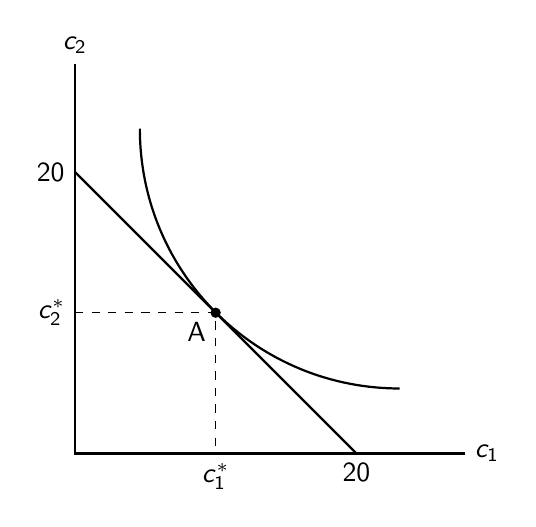
\begin{tikzpicture}[scale=0.55]
					\draw [thick] (0,6.5) node [left]{\( 20 \)} to (6.5,0) node [below]{\( 20 \)};
					\draw[thick] (0,9) node[above]{\(c_2\)} -- (0,0) -- (9,0) node[right]{\(c_1\)};
					\draw [dashed] (0,3.25) node[left]{\(c_2^*\)} -- (3.25,3.25) -- (3.25,0) node[below]{\(c_1^*\)};
					\filldraw[black] (3.25,3.25) circle (3pt) node[below left]{A};
					\draw [thick] (1.5,7.5) to [out=-90,in=180] (7.5,1.5);
				\end{tikzpicture}
				\end{figure}
			\end{explanationbox}
			\item Now look at a monetary equilibrium. Write down equations that represent the constraints on first- and second-period consumption for a typical individual. Combine these constraints into a lifetime budget constraint.
			\begin{explanationbox}
				\begin{itemize}
					\item First-period budget constraint:
					\[
						c_1 + v_tm_t \leq 20
					\]
					\item Second-period budget constraint:
					\[
						c_2 \leq v_{t+1}m_t
					\]
					\item Lifetime budget constraint:
					\[
						\frac{c_2}{v_{t+1}} \leq m_t \leq \frac{20-c_1}{v_t} \rightarrow c_1 + \frac{v_t}{v_{t+1}}c_2 \leq 20
					\]
				\end{itemize}
			\end{explanationbox}
			\item Suppose the initial old are endowed with a total of \( M = 400 \) units of fiat money. What condition represents the clearing of the money market in an arbitrary period \( t \)? Use this condition to find the real rate of return of fiat money.
			\begin{explanationbox}
				Aggregate real demand for money in period t:
				\[
					N (y-c_1) = 100 \times (20 - c_1)
				\]
				Aggregate real supply of money in period t:
				\[
					v_tM = 400v_t
				\]
			\end{explanationbox}
			\begin{explanationbox}
				The value of money is determined by the equality of money supply and money demand. Therefore, we have
				\[
					400v_t = 100 \times (20-c_1) \text{ and } v_t = \frac{100\times(20-c_1)}{400}
				\]
				Similarly,
				\[
					v_{t+1} = \frac{100\times(20-c_1)}{400}
				\]
				We can now find that the real rate of return of fiat money is
				\[
					\frac{v_{t+1}}{v_t} = \frac{\frac{100\times(20-c_1)}{400}}{\frac{100\times(20-c_1)}{400}}=1
				\]
				The value of money is constant
			\end{explanationbox}
			\item Find an individual's real demand for money. Use the assumption about preferences and your answer in part (c) to find an exact numerical value.
			\begin{explanationbox}
				In a monetary equilibrium, an individual maximizes his utility subject to the budget constraint. Mathematically,
			\begin{align*}
				\max_{c_1,c_2}\quad& c_1^{1/2} + c_2^{1/2}\\
				\text{s.t.}\quad& c_1 + c_2 = 20
			\end{align*}
			where we have substituted \( v_t=v_{t+1} \) in the budget constraint by 1. From the budget constraint, \( c_2 = 20 - c_1 \). We substitute the expression of \( c_2 \) into the utility function to have the unconstrained maximization problem:
			\[
				\max_{c_1,c_2} c_1^{1/2} + (20-c_1)^{1/2}
			\]
			The first-order condition is
			\begin{align*}
				\frac{1}{2}c_1^{-1/2}-\frac{1}{2}(20-c_1)^{-1/2}&=0\\
				c_1^{1/2} &= (20-c_1)^{-1/2}\\
				c_1 &= 20-c_1\\
				c_1 &= 10\\
				\therefore c_2 &= 10
			\end{align*}
			\end{explanationbox}
			\item What is the value of money in period \( t, v_t \)? What is the price of the consumption good \( p_t \)?
			\begin{explanationbox}
				The value of money in period \(t\) is
				\[
					v_t = \frac{100\times(20-c_1)}{400}=\frac{100\times10}{400}=2.5
				\]
				Therefore, the price level is
				\[
					p_t = \frac{1}{v_t} = \frac{1}{2.5}=0.4
				\]
			\end{explanationbox}\pagebreak
			\item Suppose instead that the initial old were endowed with a total of 800 units of fiat money. How do your answers to part (e) change? Are the initial old better off with more units of money?
			\begin{explanationbox}
				If the initial old is endowed with 800 units of money, it won't affect the choice of \((c_1,c_2)\).
				The value of money in period \(t\) is thus
				\[
					v_t = \frac{100\times(20-c_1)}{800}=\frac{100\times10}{800}=1.25
				\]
				Therefore, the price level is
				\[
					p_t = \frac{1}{v_t} = \frac{1}{1.25}=0.8
				\]
				The initial old consume \(c_2 = 10\), which is the same as before. So they are not better off with more units of money. In this economy, money is neutral. The change in the stock of money does not affect any real variables such as \( c_1 \) and \( c_2 \). Only nominal variables such as \( v_t \) and \( p_t \) are affected.\
			\end{explanationbox}
		\end{enumerate}
	\end{questionbox}
	\begin{questionbox}{Question 7}
		In this chapter, we modelled growth in an economy by a growing population. We could also achieve a growing economy by having an endowment that increases over time. To see this, consider the following economy: Let the number of young people born in each period be constant at \( N \). There is a constant stock of fiat money, \( M \). Each young person born in period \( t \) is endowed with \( y_t \) units of the consumption good when young and nothing when old. The individual endowment grows over time so that \( y_t = \alpha y_{t-1} \) where \( \alpha > 1 \). For simplicity, assume that in each period \( t \), individuals desire to hold real money balances equal to one-half of their endowment, so that \( v_tm_t = y_t= y_t/2 \).
		\begin{enumerate}[(a)]
			\item Write down equations that represent the constraints on first- and second-period consumption for a typical individual. Combine these constraints into a lifetime budget constraint.
			\begin{explanationbox}
				First-period budget constraint:
				\[
					c_1 + v_tm_t \leq y_t
				\]
				Second-period budget constraint:
				\[
					c_2 \leq v_{t+1}m_t
				\]
				Lifetime budget constraint:
				\[
					c_1+\frac{v_t}{v_{t+1}}c_2\leq y_t
				\]
			\end{explanationbox}
			\item Write down the condition that represents the clearing of the money market in an arbitrary period \( t \). Use this condition to find the real rate of return of fiat money in a monetary equilibrium. Explain the path over time of the value of fiat money.
			\begin{explanationbox}
				Aggregate real demand for money in period t:
				\[
					N (y-c_1)
				\]
				Aggregate real supply of money in period t:
				\[
					v_tM
				\]
				When money market clears, we have
				\[
					v_t=\frac{N(y_t-c_1)}{M}
				\]
				We know that the preferences are such that \( v_tm_t=\frac{y_t}{2} \). It implies that \( c_1=y_t-v_tm_t =\frac{y_t}{2}\) The value of money in period \(t\) is
				\[
					v_t=\frac{N\left(y_t-\frac{y_t}{2}\right)}{M} = \frac{Ny_t}{2M}
				\]
			\end{explanationbox}
			\begin{explanationbox}
				Similarly,
				\[
					v_{t+1} = \frac{Ny_{t+1}}{2M}
				\]
				It follows that the real rate of return of fiat money is
				\[
					\frac{v_{t+1}}{v_t} = \frac{\frac{Ny_{t+1}}{2M}}{\frac{Ny_{t+1}}{2M}} = \frac{y_{t+1}}{y_t} = \alpha
				\]
				The value of fiat money grows at a constant rate \( \alpha \) We found that in that case, the rate of return of fiat money equal to \( n \), the growth rate of the economy. In this example, \( \alpha \) is the growth rate of the economy (it is the gross rate of change of the total endowment). We discover that even in this more complicated setup, the rate of return of fiat money is equal to the growth rate of the economy when the money supply is fixed.
			\end{explanationbox}
		\end{enumerate}
	\end{questionbox}
\section{Tutorial 2}
	\begin{questionbox}{Question 1}
		According to RBA's definition of monetary aggregates, M1 includes more assets than M3 does.\\
		True, False or Uncertain. Briefly explain your answer.
		\begin{explanationbox}
			\textbf{False}. According to RBA's definition of monetary aggregates, M3 includes M1 plus all other deposits in the economy. So M3 includes more assets than M1 does.
		\end{explanationbox}
	\end{questionbox}
	\begin{questionbox}{Question 2}
		Suppose that the government increases money supply and gives new money to the old in every period. Comparing monetary equilibrium with the golden rule allocation, we find that all future generations achieve a lower level of utility but the initial old enjoys a higher level of utility in the monetary equilibrium.\\
		True, False or Uncertain. Briefly explain your answer.
		\begin{explanationbox}
			\textbf{False}. When the government increases money supply and gives new money to the old in every period, the allocation in the monetary equilibrium is not the golden rule allocation. In particular, all future generations in the monetary equilibrium achieve a lower level of utility. The initial old also achieve a lower level of utility because \( c_2 \) in the monetary equilibrium is lower than \( c_2 \) at the golden rule allocation.
		\end{explanationbox}
	\end{questionbox}
	\begin{questionbox}{Question 3}
		Suppose that the money supply grows at a constant rate \( z (z > 1) \). Comparing monetary equilibrium and the golden rule allocation, we find that individuals consume too much when young and too little when old in the monetary equilibrium.\\
		True, False or Uncertain. Briefly explain your answer.
		\begin{explanationbox}
			\textbf{True}. In a monetary equilibrium, inflation makes young individuals trade less goods for money. As a result, the old have less money to purchase goods. Comparing monetary equilibrium with the golden rule allocation, we find that individuals consume too much when young and too little when old.
		\end{explanationbox}
	\end{questionbox}
	\begin{questionbox}{Question 4}
		Suppose that the population grows at a constant rate \( n (n > 1) \) and money supply grows at a constant rate \( z (z > 1) \), the value of money falls over time.\\
		True, False or Uncertain. Briefly explain your answer.
		\begin{explanationbox}
			\textbf{Uncertain}. When the population grows at a constant rate \(n\) and money supply grows at a constant rate \(z\), we can derive money's rate of return as \(v_{t+1}/v_t = n/z\). If \(n < z\), the value of money falls over time. If \(n > z\), the value of money increases over time. And if \(n = z\), the value of money stays constant.
		\end{explanationbox}
	\end{questionbox}
	\begin{questionbox}{Question 5}
		When the population is growing, fixing the price level is the optimal policy.\\
		True, False or Uncertain. Briefly explain your answer.
		\begin{explanationbox}
			\textbf{False}. When the population is growing, money's rate of return is given by \(v_{t+1}/v_t = n/z\). The allocation in the monetary equilibrium is generally not the golden rule allocation. The optimal policy requires that an individual's budget constraint is identical to the planner's resource constraint. It implies that we need \(z=1\) for a monetary equilibrium to achieve the golden rule allocation. In this case, the value of money increases over time and the price level actually falls over time.
		\end{explanationbox}
	\end{questionbox}
	\begin{questionbox}{Question 6}
		Let \( N_t = nN_{t-1} \) and \( M_t = zM_{t-1} \) for every period \( t \), where \( z \) and  \( n \) are both greater than 1. The money created each period is used to finance a lump-sum subsidy of \( a_t^* \) goods to each young individual.
		\begin{enumerate}[(a)]
			\item Find the equation for the budget constraint of an individual in the monetary equilibrium. Graph it. Show an arbitrary indifference curve tangent to the budget constraint and indicate the levels of \( c_1 \) and \( c_2 \) that would be chosen by an individual in this equilibrium.
			\begin{explanationbox}
				First-period budget constraint:
				\[
					c_1 + v_tm_t \leq y_t + a_t^*
				\]
				Second-period budget constraint:
				\[
					c_2 \leq v_{t+1}m_t
				\]
				Lifetime budget constraint:
				\[
					c_1+\frac{v_t}{v_{t+1}}c_2\leq y_t + a_t^*
				\]
				The value of money is derived from the money market clearing condition (when aggregate money supply equals aggregate money demand),
				\begin{align*}
					v_tM_t &= N_t(y+a^*-c_1)\\
					v_t &= \frac{N_t(y+a^*-c_1)}{M_t}
				\end{align*}
				It follows that money's rate of return is
				\[
					\frac{v_{t+1}}{v_t} = \frac{\frac{N_t(y+a^*-c_1)}{M_{t+1}}}{\frac{N_t(y+a^*-c_1)}{M_t}} = \frac{N_{t+1}}{N_t} = \frac{M_{t+1}}{M_t} = \frac{n}{z}
				\]
				We can update our budget constraint as
				\[
					c_1 + \frac{n}{z}c_2 \leq y + a^*
				\]
				Graphically, we can draw the budget constraint and label point A as the allocation in a monetary equilibrium. The consumption bundle \( (c_1^*,c_2^*) \) at point A maximizes an individual's utility subject to the budget constraint.
			\end{explanationbox}
			\begin{explanationbox}
				\begin{figure}[H]
					\centering
					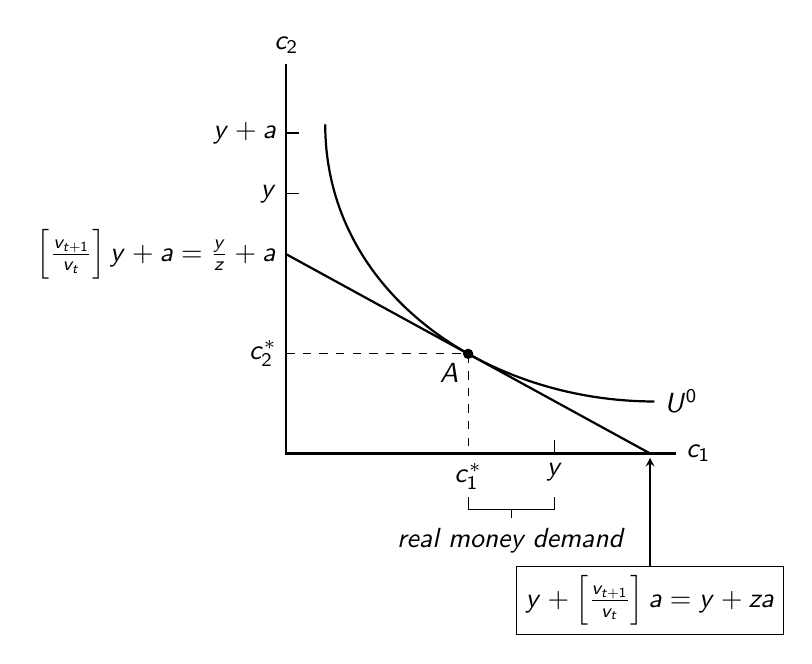
\begin{tikzpicture}[scale=0.55]
						\draw [thick] (0,4.6) node [left]{\( \left[ \frac{v_{t+1}}{v_t}  \right] y + a = \frac{y}{z} + a \)} to (8.4,0);
						\draw [->] (8.4,-2.6) node [draw, below] {\( y + \left[ \frac{v_{t+1}}{v_t} \right] a = y + za \)} -- (8.4,-0.1);
						\draw [thick] (0,9) node[above]{\(c_2\)} -- (0,0) -- (9,0) node[right]{\(c_1\)};
						\draw [dashed] (0,2.3) node[left]{\(c_2^*\)} -- (4.2,2.3) node [below left] {\( A \)} -- (4.2,0) node [below] {\(c_1^*\)};
						\draw (0,6) node [left] {\(y\)} -- (0.3,6);
						\draw (0,7.4) node [left] {\(y+a\)} -- (0.3,7.4);
						\draw (6.2,0) node [below] {\(y\)} -- (6.2,0.3);
						\draw (4.2,-1) -- (4.2,-1.3) -- (6.2,-1.3) -- (6.2,-1);
						\draw (5.2,-1.3) -- (5.2,-1.5) node [below] {\textit{real money demand}};
						\filldraw [black] (4.2,2.3) circle (3pt);
						\draw [thick] (8.5,1.2) node [right]{\( U^0 \)} to [out=-180,in=-90] (0.9,7.6) ;
					\end{tikzpicture}
				\end{figure}
			\end{explanationbox}
			\item On the graph you drew in part (a), draw the resource constraint. Take advantage of the fact that the resource constraint goes through the monetary equilibrium \( (c_1^*,c_2^*) \). Label your graph carefully, distinguishing between the budget and resource constraints.
			\begin{explanationbox}
				We first derive the resource constraint faced by the planner,
				\begin{align*}
					N_tc_1 + N_{t-1} c_2 &\leq N_t y\\
					c_1 + \frac{1}{n} c_2 &\leq y
				\end{align*}
				We add the resource constraint to the graph and label the golden rule allocation as point B.
				\begin{figure}[H]
					\centering
					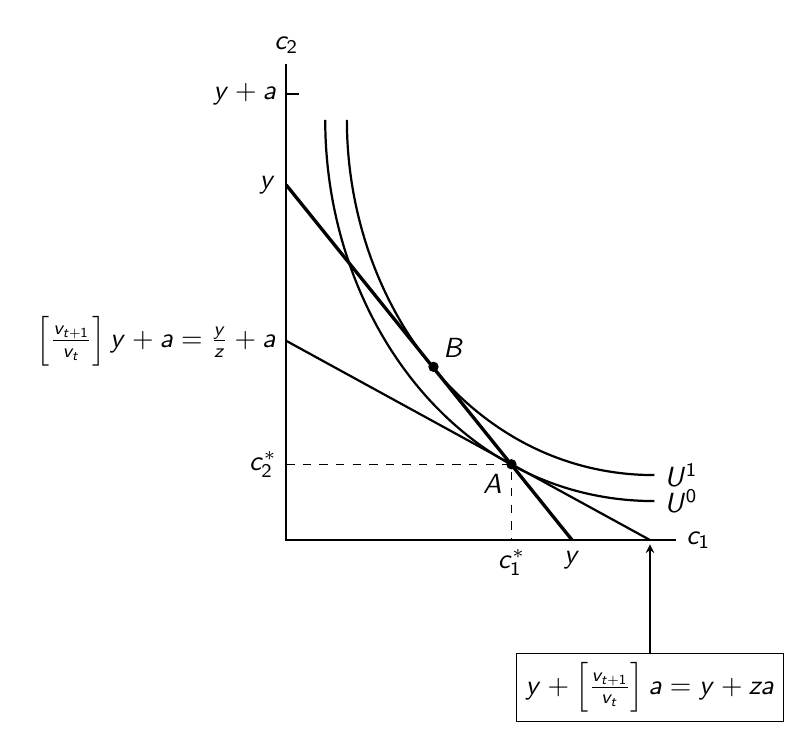
\begin{tikzpicture}[scale=0.55]
						\draw [thick] (0,4.6) node [left]{\( \left[ \frac{v_{t+1}}{v_t}  \right] y + a = \frac{y}{z} + a \)} to (8.4,0);
						\draw [->] (8.4,-2.6) node [draw, below] {\( y + \left[ \frac{v_{t+1}}{v_t} \right] a = y + za \)} -- (8.4,-0.1);
						\draw [thick] (0,11) node[above]{\(c_2\)} -- (0,0) -- (9,0) node[right]{\(c_1\)};
						\draw [dashed] (0,1.75) node[left]{\(c_2^*\)} -- (5.2,1.75) -- (5.2,0) node [below] {\(c_1^*\)};
						\draw [very thick] (0,8.2) node [left] {\(y\)} -- (6.6,0) node [below] {\(y\)};
						\draw (0,10.3) node [left] {\(y+a\)} -- (0.3,10.3);
						\draw [thick] (8.5,0.9) node [right]{\( U^0 \)} to [out=-180,in=-90] (0.9,9.7);
						\draw [thick] (8.5,1.5) node [right]{\( U^1 \)} to [out=-180,in=-90] (1.4,9.7);
						\filldraw [black] (3.4,4) circle (3pt) node [above right] {\( B \)};
						\filldraw [black] (5.2,1.75) circle (3pt) node [below left] {\( A \)};
					\end{tikzpicture}
				\end{figure}
			\end{explanationbox}\pagebreak
			\item Show that the monetary equilibrium does not maximize the utility of the future generations. Support your assertion with references to the graph you drew of the budget and feasible constraints.
			\begin{explanationbox}
				We can clearly see from the graph that there are feasible points that are preferred by the future generations to \( (c_1^*,c_2^*) \). One such point is point B which is the golden rule allocation. Point B lies on a higher indifference curve than \( (c_1^*,c_2^*) \). This shows that given the resource constraint (or feasible constraint), the stationary monetary equilibrium \( (c_1^*,c_2^*) \) does not maximize the utility of future generations. Furthermore, the initial old also prefer a point like A since it gives them higher second-period consumption than \( c_2^* \).
			\end{explanationbox}
		\end{enumerate}
	\end{questionbox}
	\begin{questionbox}{Question 7}
		Consider an overlapping generations model with the following characteristics: Each generation is composed of 1,000 individuals. The money supply changes according to \( M_t = 2M_{t-1} \). The initial old own a total of 10,000 units of money \( M_0 = \$10,000 \). Each period, the newly printed money is given to the old of that period as a lump-sum transfer. Each individual is endowed with 20 units of the consumption good when born and nothing when old. Preferences are such that individuals wish to save 10 units when young at the equilibrium rate of return on money.
		\begin{enumerate}[(a)]
			\item What is the gross real rate of return on money in this economy \( (\frac{v_{t+1}}{v_t}) \)?
			\begin{explanationbox}
				To derive the rate return on money, we first need to find the value of money. The money market clearing condition is
				\begin{align*}
					v_tM_t &= N(y-c_1)\\
					v_t &= \frac{N(y-c_1)}{M_t}
				\end{align*}
				It follows that
				\[
					\frac{v_{t+1}}{v_t} = \frac{\frac{N(y-c_1)}{M_{t+1}}}{\frac{N(y-c_1)}{M_t}} = \frac{M_{t+1}}{M_t} = \frac{1}{2}
				\]
				The rate of return on money is \( \frac{1}{2} \). The value of money falls by a half every period.
			\end{explanationbox}
			\item How many goods does an individual consume when young \( (c_1) \)?
			\begin{explanationbox}
				Individuals allocate their endowments between consumption and saving when young.\\
				The first-period budget constraint is
				\[
					c_1 + v_tm_t \leq y
				\]
				When individuals save 10 units when young, it means that \( v_tm_t = 10 \). Given that \( y=20 \), we have \( c_1 = y-v_tm_t = 10 \). The consumption when young is 10 units of good
			\end{explanationbox}
			\item How many goods does an individual receive as a transfer \( (a) \)?
			\begin{explanationbox}
				From the government budget constraint, the transfer is from the newly printed money.\\
				In aggregate,
				\[
					Na = v_t(M_t-M_{t-1}) = v_t \left( M_t-\frac{M_t}{2} \right) = \frac{1}{2} v_tM_t.
				\]
				To find the value of \( v_tM_t \), we use the money market clearing condition
				\[
					v_tM_t = N(y-c_1) = 1000 \times (20-10) = 10,000
				\]
				It follows that the amount of the transfer in real terms is given by
				\[
					a = \frac{\frac{1}{2}v_tM_t}{N} = \frac{\frac{1}{2}\times 10,000}{1000} =  5
				\]
			\end{explanationbox}
			\item How many goods does an individual consume when old \( (c_2) \)?
			\begin{explanationbox}
				From an individual's second-period budget constraint,
				\[
					c_2 \leq v_{t+1}m_t + a
				\]
				Recall that \( v_tm_t = 10 \). We can derive the value of \( v_{t+1}m_t \) as
				\[
					v_{t+1}m_t = \frac{1}{2} \times 10 = 5
				\]
				Therefore, we have
				\begin{align*}
					c_2 &= v_{t+1}m_t + a\\
					&= 5 + 5 = 10
				\end{align*}
				The second-period consumption is 10 units of good. 
			\end{explanationbox}
			\item What is the price of the consumption good in period 1 in dollars \( (p_1) \)?
			\begin{explanationbox}
				The price is the inverse of the value of money,
				\[
					p_1 = \frac{1}{v_1}
				\]
				We will find the value of \( v_1 \). Given that
				\[
					v_t = \frac{N(y-c_1)}{M_t},
				\]
				we have
				\[
					v_1 = \frac{N(y-c_1)}{M_1} = \frac{1000 \times (20-10)}{2 \times M_0} = \frac{1000 \times 10}{2 \times 10000} = \frac{1}{2}
				\]
				Finally, the price level in period 1 is
				\[
					p_1 = \frac{1}{v_1} = 2
				\]
			\end{explanationbox}
		\end{enumerate}
	\end{questionbox}
\section{Tutorial 3}
	\begin{questionbox}{Question 1}
		Suppose that the government creates new money to finance its own purchases. Comparing monetary equilibrium and the golden rule allocation, we find that both \( c_1 \) are \( c_2 \) are lower in a monetary equilibrium than at the golden rule allocation.\\
		True, False or Uncertain. Briefly explain your answer.
		\begin{explanationbox}
			\textbf{False.} In a monetary equilibrium, young individuals would choose to trade less goods for money when money supply is growing. As a result, the old consume less but the young consume more compared to the golden rule allocation. That is, \( c_1 \) is higher and \( c_2 \) is lower in a monetary equilibrium.
		\end{explanationbox}
	\end{questionbox}
	\begin{questionbox}{Question 2}
		To finance the same amount of government purchases, using a lump-sum tax is better than using the inflation tax (money creation).\\
		True, False or Uncertain. Briefly explain your answer.
		\begin{explanationbox}
			\textbf{Uncertain.} When using the in‡ation tax to finance government purchases, we know that the allocation in the monetary equilibrium achieves a lower level utility than the golden rule allocation. If the government uses a lump-sum tax instead of the in‡ation tax, it is possible to design the lump-sum tax such that the allocation in the monetary equilibrium can coincide with the golden rule allocation. In particular, it requires that the government keeps a constant money supply and sets the per capita lump-sum tax to the per capita government purchases.
		\end{explanationbox}
	\end{questionbox}
	\begin{questionbox}{Question 3}
		In most countries, seigniorage contributes significantly to total government revenue.\\
		True, False or Uncertain. Briefly explain your answer.
		\begin{explanationbox}
			\textbf{False.} In most industrialized countries during normal times, seigniorage contributes to total government revenue, but it accounts for only a small fraction of total government revenue. However, for countries that experience high in‡ation episodes, seigniorage could contribute significantly to total government revenue.
		\end{explanationbox}
	\end{questionbox}
	\begin{questionbox}{Question 4}
		The government can finance any amount of government purchases by creating new money.\\
		True, False or Uncertain. Briefly explain your answer.
		\begin{explanationbox}
			\textbf{False.} When the government creates new money to finance its own purchases, a higher growth rate of money supply does not always lead to a higher level of seigniorage in real terms. A higher growth rate of money supply means that a higher fraction of real value of money stock will be collected by the government. However, the real value of the total money stock decreases when the growth rate of money supply increases. Overall, when the growth rate of money supply is low, a higher growth rate leads to more seigniorage. When the growth rate of money supply is high, a higher growth rate leads to less seigniorage.
		\end{explanationbox}
	\end{questionbox}
	\begin{questionbox}{Question 5}
		Assume that people face a lump-sum tax of \( \tau \) goods when old and a growth rate of money supply of \( z > 1 \). The tax and the newly created money are used to finance government purchases of \( g \) goods per young individual in very period. There are \( N \) individuals in every generation.
		\begin{enumerate}[(a)]
			\item Find the individual's budget constraints when young and when old. Combine them to form the individual's lifetime budget constraint and graph this constraint.
			\begin{explanationbox}
				First period budget constraint:
				\[
					c_{1,t} + v_t m_t \leq y
				\]
				Second period budget constraint:
				\[
					c_{2,t+1} \leq v_{t+1} m_t - \tau
				\]
				Lifetime budget constraint:
				\[
					c_1 + \frac{v_{t+1}}{v_t} c_2 \leq y - \frac{v_{t+1}}{v_t} \tau
				\]
				Money market clearing condition:
				\begin{align*}
					m_t v_t &= N (y-c_1) \\
					v_t &= \frac{N(y-c_1)}{M_t}
				\end{align*}
			\end{explanationbox}
			\begin{explanationbox}
				We can then derive money's rate of return as
				\begin{gather*}
					\frac{v_{t+1}}{v_t} = \frac{\frac{N_{t+1} (y-c_1)}{M_{t+1}}}{\frac{N_t (y-c_1)}{M_t}} = \frac{M_t}{M_{t+1}} = \frac{M_t}{zM_t} = \frac{1}{z} < 1 \\
					\Rightarrow \frac{v_t}{v_{t+1}} = z
				\end{gather*}
				Updated individual's budget constraint:
				\[ 
					c_1 + zc_2 \leq y - z \tau 
				\]
				\begin{figure}[H]
					\centering
					\begin{tikzpicture}[scale=0.55]
						\draw [thick] (0,4.6) node [left]{\( \frac{y}{z}-\tau \)} to (8.4,0) node [below] {\( y-z\tau \)};
						\draw[thick] (0,9) node[above]{\(c_2\)} -- (0,0) -- (9,0) node[right]{\(c_1\)};
					\end{tikzpicture}
				\end{figure}
			\end{explanationbox}
			\item Find the government's budget constraint.
			\begin{explanationbox}
				The government's budget constraint is
				\begin{align*}
					g &= \tau + \frac{(M_t-M_{t-1})v_t}{N}\\
					&= \tau + \frac{(1-\frac{1}{z})M_tv_t}{N}\\
					\intertext{Using the money market clearing condition we have:}
					&= \tau + \frac{(1-\frac{1}{z})N(y-c_1)}{N}\\
					&= \tau + \left( 1-\frac{1}{z} \right) (y-c_1)
				\end{align*}	
			\end{explanationbox}
			\item Graph the stationary monetary equilibrium.
			\begin{explanationbox}
				The stationary monetary equilibrium can be found at the tangency point between the indifference curve and the individual's budget constraint. Point A in the figure below mrepresents the allocation in the monetary equilibrium
			\end{explanationbox}
			\begin{explanationbox}
				\begin{figure}[H]
					\centering
					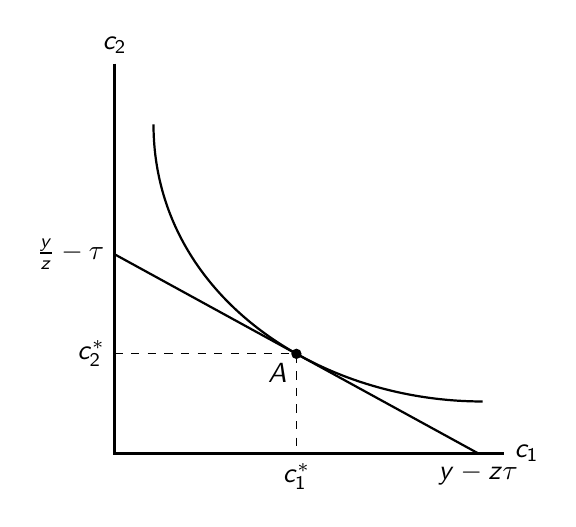
\begin{tikzpicture}[scale=0.55]
						\draw [thick] (0,4.6) node [left]{\( \frac{y}{z}-\tau \)} to (8.4,0) node [below] {\( y-z\tau \)};
						\draw [thick] (0,9) node[above]{\(c_2\)} -- (0,0) -- (9,0) node[right]{\(c_1\)};
						\draw [dashed] (0,2.3) node[left]{\(c_2^*\)} -- (4.2,2.3) -- (4.2,0) node [below] {\(c_1^*\)};
						\filldraw [black] (4.2,2.3) circle (3pt) node [below left]{\( A \)};
						\draw [thick] (8.5,1.2) to [out=-180,in=-90] (0.9,7.6);
					\end{tikzpicture}
				\end{figure}
			\end{explanationbox}
			\item Find the stationary monetary equilibrium when \( z = 1 \) and add it to the graph in (c)
			\begin{explanationbox}
				When \( z=1 \), the individual’s budget constraint is
				\[
				c_1+c_2\leq y-\tau	
				\]
				We graph the budget constraint and find the allocation in a monetary equilibrium at point B when z = 1.
				\begin{figure}[H]
					\centering
					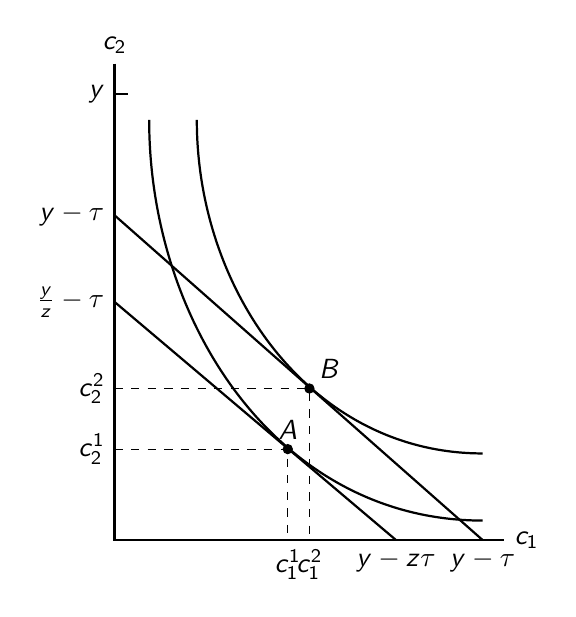
\begin{tikzpicture}[scale=0.55]
						\draw [thick] (0,5.5) node [left]{\( \frac{y}{z}-\tau \)} to (6.5,0) node [below] {\( y-z\tau \)};
						\draw [thick] (0,7.5) node [left]{\( y-\tau \)} to (8.5,0) node [below] {\( y-\tau \)};
						\draw [thick] (0,11) node[above]{\(c_2\)} -- (0,0) -- (9,0) node[right]{\(c_1\)};
						\draw (0,10.3) node [left] {\(y\)} -- (0.3,10.3);
						\draw [thick] (8.5,0.45) to [out=-180,in=-90] (0.8,9.7);
						\draw [thick] (8.5,2) to [out=-180,in=-90] (1.9,9.7);
						\filldraw [black] (4.5,3.5) circle (3pt) node [above right] {\( B \)};
						\draw [dashed] (0,3.5) node [left] {\( c_2^2 \)}-- (4.5,3.5) -- (4.5,0) node [below] {\( c_1^2 \)};
						\filldraw [black] (4,2.1) circle (3pt) node [above] {\( A \)};
						\draw [dashed] (0,2.1) node [left] {\( c_2^1 \)}-- (4,2.1) -- (4,0) node [below] {\( c_1^1 \)};
					\end{tikzpicture}
				\end{figure}
			\end{explanationbox}
			\item Compare the real balances of fiat money when \( z > 1 \) to the value when \( z = 1 \).
			\begin{explanationbox}
				Comparing \( c_1 \) when \( z > 1 \) and when \( z = 1 \), we find that the \( c_1 \) is higher when \( z > 1 \) than when \( z = 1 \). Since the real money balances held by any individual is
				\[
					v_tm_t = y - c_1
				\]
				the real money balances of money is lower when \( z > 1 \) than when \( z = 1 \). That is, a higher growth rate of money supply reduces the real money balances held by any individual. As a result, the aggregate real money balances in the economy also decline as \( z \) increases.
			\end{explanationbox}\pagebreak
			\item What is the optimal choice of \( (\tau, z) \) so that individuals achieve the highest level of utility?
			\begin{explanationbox}
				To achieve the highest level of utility, the allocation of \( (c_1,c_2) \) should be the golden rule allocation. The golden rule allocation can be found when the planner maximizes an individual’s utility subject to the economy's resource constraint. In this economy, the resource constraint is
				\[
					c_1+c_2 \leq y - g
				\]
				where \( g \) is the per capita government purchases. For the optimal policy, the government chooses \( \tau, z \) so that the individual’s budget constraint can coincide with the resource constraint. The optimal policy is to let \( \tau = g \)	and \( z = 1 \).
			\end{explanationbox}
		\end{enumerate}
	\end{questionbox}
	\begin{questionbox}{Question 6}
		Consider an economy with a constant population of \( N = 1000 \). Individuals are endowed with \( y = 20 \) units of the consumption good when young and nothing when old. All seigniorage revenue is used to finance government expenditures. There are no subsidies and no taxes other than seigniorage. Suppose that preferences are such that each individual wishes to hold real balances of fiat money worth
		\[
			\frac{y}{1 + \frac{v_t}{v_{t+1}}}
		\]
		goods
		\begin{enumerate}[(a)]
			\item Use the equality of supply and demand in the money market to find the total real balances of fiat money in a stationary equilibrium as a function of the rate of fiat money creation \( z \).
			\begin{explanationbox}
				The total real balances of money is
				\[
					v_tM_t
				\]
				The money market clearing condition implies that
				\[
					v_tM_t = N(y-c_1)
				\]
				The value of money in period t is then
				\[
					v_t = \frac{N(y-c_1)}{M_t}
				\]
				Money's rate of return is
				\[
					\frac{v_{t+1}}{v_t} = \frac{\frac{N(y-c_1)}{M_{t+1}}}{\frac{N(y-c_1)}{M_t}} = \frac{M_t}{M_{t+1}} = \frac{1}{z}
				\]
				The amount of money in real terms that each young individual chooses to hold is
				\begin{align*}
					v_tm_t = y - c_1 &= \frac{y}{1 + \frac{v_t}{v_{t+1}}}\\
					&= \frac{y}{1 + z}
				\end{align*}
				Therefore, the total real balances of money as a function of \( z \) is
				\begin{align*}
					v_tM_t &= N(y-c_1)\\
					&= N\frac{y}{1 - z}\\
					&= \frac{1000 \times 20}{1 + z}\\
					&= \frac{20,000}{1 + z}
				\end{align*}
				We can see that a higher \( z \) leads to a lower \( v_tM_t \).
			\end{explanationbox}\pagebreak
			\item Use your answer in part (a) to find total seigniorage revenue as a function of \( z \). Graph this function and explain its shape.
			\begin{explanationbox}
				The total seigniorage revenue in real terms is
				\[
					G = (M_t - M_{t-1})v_t = \left( 1 - \frac{1}{z} \right) M_tv_t
				\]
				Using the solution of \( v_tM_t \) that we found in part (a), we have
				\begin{align*}
					G &= \left( 1 - \frac{1}{z} \right) \frac{20,000}{1+z}\\
					&= 20,000\frac{1-\frac{1}{z}}{1+z}
				\end{align*}
				\begin{figure}[H] \centering
					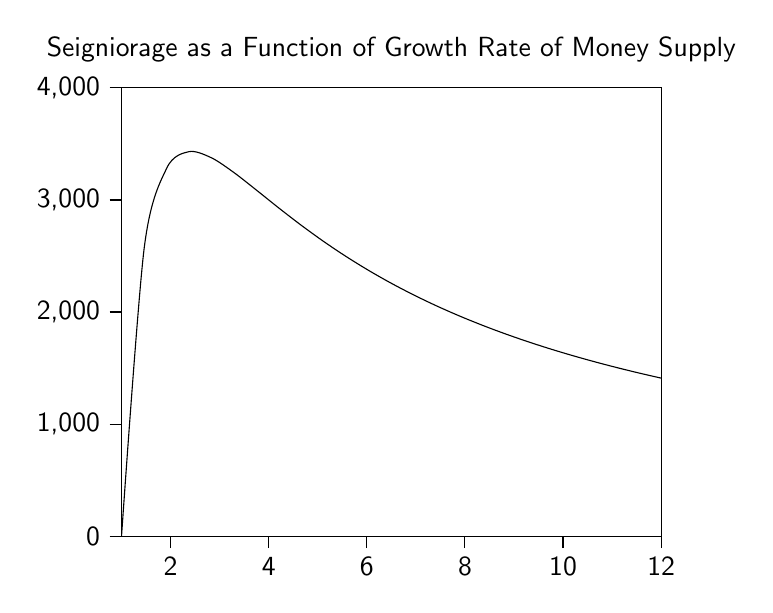
\begin{tikzpicture}
						\begin{axis}[
							title = {Seigniorage as a Function of Growth Rate of Money Supply},
							axis on top,
							no markers,
							xmin = 1,
							xmax = 12,
							xtick pos = left,
							xtick align = outside,
							ytick pos = bottom,
							ytick align = outside,
							ymin = 0,
							ymax = 4000,
							]
							\addplot+[black, smooth, no markers, domain=1:12] {20000*((1-(1/x))/(1+x))};
						\end{axis}
					\end{tikzpicture}
				\end{figure}
			\end{explanationbox}
		\end{enumerate}
	\end{questionbox}
\section{Tutorial 4}
	\begin{questionbox}{Question 1}
		The correlation between inflation and unemployment in the original Phillips curve is consistent with cross country evidence on the correlation between inflation and output growth.\\
		True, False or Uncertain. Briefly explain your answer.
		\begin{explanationbox}
			\textbf{False}. The original Phillips curve finds that there is a negative correlation between inflation and unemployment, which means that higher inflation is associated with more em-ployment and output. However, cross country evidence suggests that on average, countries with high inflation rates are associated with lower output growth. This is inconsistent with the prediction from the original Phillips curve.
		\end{explanationbox}
	\end{questionbox}
	\begin{questionbox}{Question 2}
		In the Lucas model, the current price of the good is higher on the island with less young individuals.\\
		True, False or Uncertain. Briefly explain your answer.
		\begin{explanationbox}
			\textbf{True}. On the island with less young individuals, there are less young individuals supplying labor to produce the goods. The relative less supply of the goods leads to a higher price of the goods compared with the island with more young individuals.
		\end{explanationbox}
	\end{questionbox}
	\begin{questionbox}{Question 3}
		In the Lucas model, when monetary policy is not random (i.e., the growth rate of money supply is constant), the young cannot infer the true state of the world (i.e., the island where they live and the current money supply) from the prices.\\
		True, False or Uncertain. Briefly explain your answer.
		\begin{explanationbox}
			\textbf{False}. It is true that the young individuals in the Lucas model do not know the current money supply and the distribution of the young population across the two islands. However, they are rational, which means that they will make the most correct inference from the information they have. When money supply grows at a constant rate, individuals can infer the current money supply from last period's money supply and the growth rate of money supply. Individuals can also infer whether they live on the island with less young individuals or more young individuals through the prices. They know that there should exist two prices. In addition, they know that the high price should occur on the island with less young individuals and the low price should occur on the island with more young individuals. Overall, the young can infer the true state of the world from the information that they have when monetary policy is not random.
		\end{explanationbox}
	\end{questionbox}
	\begin{questionbox}{Question 4}
		Money is superneutral in the Lucas Model\\
		True, False or Uncertain. Briefly explain your answer.
		\begin{explanationbox}
			\textbf{False}. In the Lucas model, when the growth rate of money supply increases, the rate of return to labor decreases. As a result, labor supply will decrease and output will decrease. The increase in the growth rate of money supply affects real variables such as labor supply and output in the model. When the change in the growth rate of money supply affects real economic variables in a model, we say that money is not superneutral.
		\end{explanationbox}
	\end{questionbox}
	\begin{questionbox}{Question 5}
		In the Lucas model, when monetary policy is random, the young cannot infer the true state of the world from the prices.\\
		True, False or Uncertain. Briefly explain your answer.
		\begin{explanationbox}
			\textbf{True/Uncertain}. Then the growth rate of money supply is random, the young can no longer infer the current money supply and the distribution of young individuals from the prices. In the model we showed in class, there are potentially four prices. Two of the prices are unique and individuals can infer the true state from these two prices. However, the other two prices are the same. It means that individuals cannot tell whether they are on the island with less young individuals and a lower growth rate of money supply or they are on the island with more young individuals and a higher growth rate of money supply. Overall, the young cannot infer the true state of the world from the information they have when monetary policy is random.
		\end{explanationbox}
	\end{questionbox}
	\begin{questionbox}{Question 6}
		Consider the following version of the Lucas model. The number of young individuals born on island \( i \) in period \( t \); \( N_t^i \) is random according to the following specification:
		\begin{alignat*}{2}
			N_t^i &= \frac{4}{5}N &\quad&\text{with probability 0.5} \\
			&= \frac{1}{5}N &\quad&\text{with probability 0.5}
		\end{alignat*}
		Assume that the money supply grows at the constant rate \( z_t = z \) in all periods.
		\begin{enumerate}[(a)]
			\item Set up the budget constraints of the individuals when young and when old. Also set up the government budget constraint and money market clearing condition. Find the lifetime budget constraint (combine the budget constraints of the young and old).
			\begin{explanationbox}
				Budget constraint for the young:
				\begin{gather*}
					c_{1,t}^i + l_t^i \leq y\\
					c_{1,t}^i +  v_t^i m_t^i \leq y
				\end{gather*}
				Budget constraint for the old:
				\begin{align*}
					c_{2,t+1}^{i,{\,j}} &\leq v_{t+1}^{\,j} m_t^i + a_{t+1^{}}\\
				\end{align*}
				Budget constraint for the government:
				\[
					N_{t-1} a_t \leq (M_t - M_{t-1}) v_t = (1-\frac{1}{z})M_t v_t
				\]
				Inter-temporal Budget constraint:
				\[
					c_{1,t}^i  + \frac{v_t^i}{v_{t+1}^{\,j}}c_{2,t+1}^{i,\,j} \leq y +  \frac{v_t^i}{v_{t+1}^{\,j}} + a_{t+1^{}}
				\]
				Money market clearing condition:
				\begin{align*}
					N_t^i \left( y-c_{1,t}^i \right) &= v_t^i \frac{M_t}{2} \\
					N_t^i l_t^i &= v_t^i\frac{M_t}{2}
				\end{align*}
			\end{explanationbox}
			\item On which island would you prefer to be born? Explain with reference to the rate of return to labour.
			\begin{explanationbox}
				You would want to be born on the island with the greatest rate of return to labor. In this model, the rate of return to labor is
				\[
					\frac{v_{t+1}^{\,j}}{v_t^i} = \frac{p_t^i}{p_{t+1}^{\,j}}
				\]
				Assuming substitution effect dominates income effect;
				\begin{gather*}
					p_t^a = \frac{\frac{M_t}{2}}{N^A l_t^A} = \frac{\frac{M_t}{2}}{\frac{1}{5}N l_t^A}\\ 
					p_t^b = \frac{\frac{M_t}{2}}{N^B l_t^B} = \frac{\frac{M_t}{2}}{\frac{2}{5}N l_t^B}
				\end{gather*}
				\( p_t^A > p_t^B \) the price level is higher on the island with less young individual. Intuition: when there are less young people, there are less people supplying labour to produce the good. With the same number of old individuals, the demand for goods is relatively high on the island with less young individuals. Therefore, the price is high on the island with less young individuals.
			\end{explanationbox}
			\item Show how the rate of return to labour and the individual's labour supply depend on the value of \( z \).
			\begin{explanationbox}
				Here the growth rate of money supply is constant. The rate of return to labor is
				\[
					\frac{v_{t+1}^{\,j}}{v_t^i} = \frac{p_t^i}{p_{t+1}^{\,j}} = \frac{\frac{M_t/2}{N^i l_t^i}}{\frac{M_{t+1} / 2}{N^j l_{t+1}^{\,j}}} = \frac{N^j l_{t+1}^{\,j}}{N^i l_t^i} \frac{M_t}{M_{t+1}}=\frac{N^j l_{t+1}^{\,j}}{N^i l_t^i} \frac{1}{z}
				\]
			\end{explanationbox}
			\begin{explanationbox}
				We can clearly see from this equation that as the value of z increases, the rate of return to labor falls. Such a change will generate a decline in labor supply and hence lower output.
			\end{explanationbox}
		\end{enumerate}
		For the following parts, assume that the growth rate of money supply \( z_t \) is random according to
		\begin{alignat*}{2}
			z_t &= 1 &\quad&\text{with probability } \theta \\
			&= 4 &\quad&\text{with probability } 1- \theta
		\end{alignat*}
		The realisation of \( z_t \) is kept secret from the young until all purchases of goods have occurred (i.e., individuals do not learn \( M_t \) until period \( t \) is over). Given these changes in assumption, answer the following questions:
		\begin{enumerate}[(a), resume]
			\item How many states of the world would individuals be able to observe if information about every variable were perfectly available? Describe those possible states.
			\begin{explanationbox}
				If agents could perfectly observe information about every variable, there would be four states of the world, corresponding to four combinations of \(N_t^i\) and \(z_t\). See below for the prices corresponding to the four states.
				\begin{table}[H]
					\centering
					\renewcommand{\arraystretch}{1.5}
					\begin{tabular}{c|cc} \hhline{===}
						& \( \frac{4}{5} N \) & \( \frac{1}{5} N \) \\ \hline
						\( z_t = 1 \) & \( p_t^a = \frac{M_{t-1} / 2}{\frac{4}{5} N l (p_t^a)} \) & \( p_t^b = \frac{M_{t-1} / 2}{\frac{1}{5} N l (p_t^b)} \) \\
						\( z_t = 4 \) & \( p_t^c = \frac{4M_{t-1} / 2}{\frac{4}{5} N l (p_t^c)} \) & \( p_t^d = \frac{4M_{t-1} / 2}{\frac{1}{5} N l (p_t^d)} \) \\ [3pt] \hhline{===}
					\end{tabular}
				\end{table}
			\end{explanationbox}
			\item How many states of the world are the individuals able to distinguish when there is limited information (i.e., they do not know the value of \( z_t \))
			\begin{explanationbox}
				If individuals do not observe \(z_t\) and \(N^i\), two out of four prices would be unique so that individuals can still distinguish. The rest two prices will look the same to individuals. In above table, \(p_t^a < p_t^b = p_t^c < p_t^d\). If individuals observe \(p_t^a\) or \(p_t^d\), they will be able to infer the current \(z_t\) and \(N^i\). However, \(p_t^b\) and \(p_t^c\) are the same. Individuals will not be able to distinguish between state \(b\) where \(Ni = N/5\) and \(z_t = 1\) versus state \(c\) where \(N^i = 4N/5\) and \(z_t = 4\).
			\end{explanationbox}
			\item Draw a graph of labour supply and the growth rate of money supply in each possible state of the world when there is limited information. What is the correlation observed between money creation and output?
			\begin{explanationbox}
				If the price \(p_t^a\) is observed, individuals know that they are on the island with more young individuals and a lower growth rate of money. The low current price leads to a lower level of labour supply \( l_t^a \) If price \( p^d_t \) is observed, individuals know that they are on the island with less young individuals and a higher growth rate of money supply. The high current price leads to a higher level of labor supply \( l_t^d \). Individuals cannot distinguish between state \( b \) and \( c \). When they observe \(p_t^b\) or \(p_t^c\), they are not sure whether they are on the island with less young individuals and a lower growth rate of money supply or they are on the island with more young individuals and a higher growth rate of money supply. Each individual will supply an intermediate level of labor \( l^* \). Overall, \(l_t^a < l^* < l_t^d\). There appears to be a positive correlation between money creation and output.
			\end{explanationbox}
			\begin{explanationbox}
				\begin{figure}[H]
					\centering
					\begin{tikzpicture}[scale=0.55]
						\draw[thick] (0,9) node[above]{\(z\)} -- (0,0) -- (9,0) node[right]{\(l / L\)};
						\draw (0,6) node [left] {\(4\)} -- (0.3,6);
						\draw (0,3) node [left] {\(1\)} -- (0.3,3);
						\draw (2.5,0) node [below] {\(l^a\)} -- (2.5,0.3);
						\draw (4.5,0) node [below] {\(l^*\)} -- (4.5,0.3);
						\draw (6.5,0) node [below] {\(l^b\)} -- (6.5,0.3);
						\node at (2.5,3) {\( a \)};
						\node at (4.5,3) {\( b \)};
						\node at (4.5,6) {\( c \)};
						\node at (6.5,6) {\( d \)};
					\end{tikzpicture}
				\end{figure}	
			\end{explanationbox}
			\item Suppose the government wanted to take advantage of the relation between money creation and output. If it always inflate \( (\theta = 0) \), will the graph you derived in part (f) remain the same. Explain your answer.
			\begin{explanationbox}
				If the government always inflate, there will be no randomness to inflation. Individuals will no longer be confused about the world. Only state \(c\) and \(d\) will exist. They know that \(z = 4\). When individuals observe a high price, they know they are on an island with less young individuals. When individuals observe a low price, they know they are on an island with more young individuals. Compared with the level of output at \(z = 1\), output produced at \(z = 4\) is lower because the higher growth rate of money supply lowers the rate of return to labour and hence labour supply and output fall. The positive correlation between money creation and output disappears when the government tries to exploit it.
			\end{explanationbox}
		\end{enumerate}
	\end{questionbox}
\section{Tutorial 5}
	\begin{questionbox}{Question 1}
		The Lucas Critique stresses that the government cannot design policy purely based on the reduced form correlation from the data.\\
		True, False or Uncertain. Briefly explain your answer.
		\begin{explanationbox}
			\textbf{True.} The Lucas Critique points out that the reduced form correlations are subject to change when the government changes its policies and thus the rules under which decision makers operate. It implies that while econometric policy evaluation is useful, we also need a theory to help us understand how people react to different government policies. It is not sufficient just to look at the data.
		\end{explanationbox}
	\end{questionbox}
	\begin{questionbox}{Question 2}
		In an OLG model with two countries and two monies/currencies, people would like to hold both currencies no matter what the values of these currencies are.\\
		True, False or Uncertain. Briefly explain your answer.
		\begin{explanationbox}
			\textbf{False.} When people are free to hold and use any currency, people would choose to hold the currency (or currencies) that can help them buy the most goods. In equilibrium, only when the exchange rate satisfies \( e_t=v_t^a/v_t^b \) both currencies are valued and held by people.
		\end{explanationbox}
	\end{questionbox}
	\begin{questionbox}{Question 3}
		In an OLG model with two countries and two currencies, suppose that foreign currency controls are in effect. The government cannot choose to both fix the exchange rate and acquire its preferred level of seigniorage.\\
		True, False or Uncertain. Briefly explain your answer.
		\begin{explanationbox}
			\textbf{True.} When foreign currency controls are in effect, the government has to set its growth rate of money supply according to \(za = z^bn^a/n^b\) to keep a fixed exchange rate. In this case, the government cannot freely choose its preferred level of seigniorage. If the government wants to choose \(z^a\) to generate a certain level of seigniorage, the exchange rate cannot be fixed. Overall, it is not possible to both fix the exchange rate and acquire a preferred level of seigniorage when foreign currency controls are in effect.
		\end{explanationbox}
	\end{questionbox}
	\begin{questionbox}{Question 4}
		The fluctuations in exchange rates can always be attributed to changes in economic fundamentals.\\
		True, False or Uncertain. Briefly explain your answer.
		\begin{explanationbox}
			\textbf{False.} From the data on exchange rate fluctuations, we can see a lot of extreme fluctuations cannot be tied to any changes in real economic conditions. Neither the change in money supply nor the change in money demand can explain the change in exchange rate. Fluctuations in exchange rates cannot always be attributed to changes in economic fundamentals.
		\end{explanationbox}
	\end{questionbox}
	\begin{questionbox}{Question 5}
		In an OLG model with international currency traders, there exist two money market clearing conditions for the two monies. Therefore, the exchange rate is no longer indeterminate.\\
		True, False or Uncertain. Briefly explain your answer.
		\begin{explanationbox}
			\textbf{False.} Even if there are two money market clearing conditions, exchange rate is still indeterminate as long as international currency traders can freely adjust its holding of different currencies. Basically, whenever international currency traders changes the composition of their currency portfolios, it will change the exchange rate.
		\end{explanationbox}
	\end{questionbox}
	\begin{questionbox}{Question 6}
		Suppose that the United States (country \( a \)) and Great Britain (country \( b \)) have foreign currency controls in effect. The demand for money is growing at 10.25 percent in the United States and at 2 percent in Great Britain (net rates) each period. The money supplies in the United States and Britain are growing at 5 and 6.25 percent (net rates) in each period, respectively.
		\begin{enumerate}[(a)]
			\item Define the exchange rate (\( e_t \)) as in our lectures, what are the units in which the exchange rate is measured, U.S. dollars per British pound or British pounds per U.S. dollar?
			\begin{explanationbox}
				Exchange rate:
				\[
					e_t = \frac{\text{units of British pounds}}{\text{units of U.S dollar}}
				\]
			\end{explanationbox}
			\item What is the rate of return on money in the U.S.? In Great Britain?
			\begin{explanationbox}
				The rate of return on money in the U.S. can be expressed as
				\[
					\frac{v_{t+1}^a}{v_t^a} = \frac{\frac{N_{t+1}^a \left( y^a - c_1^a \right)}{M_{t+1}^a}}{\frac{N_t^a \left( y^a - c_1^a \right)}{M_t^a}} = \frac{N_{t+1}^a}{N_t^a}\frac{M_t^a}{M_{t+1}^a} = \frac{n^a}{z^a} = \frac{1.1025}{1.05} = 1.05
				\]
			\end{explanationbox}
			\begin{explanationbox}
				The rate of return on money in Great Britain can be expressed as
				\[
					\frac{v_{t+1}^b}{v_t^b} = \frac{\frac{N_{t+1}^b \left( y^b - c_1^b \right)}{M_{t+1}^b}}{\frac{N_t^b \left( y^b - c_1^b \right)}{M_t^b}} = \frac{N_{t+1}^b}{N_t^b}\frac{M_t^b}{M_{t+1}^b} = \frac{n^b}{z^b} = \frac{1.02}{1.0625} = 0.96
				\]
				The exchange rate is increasing over time, since the real value of U.S. dollar is increasing over time whereas that of British pounds is decreasing over time. It implies that the relative value of the U.S. dollar to the British pound is increasing over time.
			\end{explanationbox}
			\item In a system of flexible exchange rate, what is the time path of the exchange rate between the U.S. and Great Britain \( (e_{t+1}/e_t) \)
			\begin{explanationbox}
				For exchange rate:
				\begin{gather*}
					e_t = \frac{v_t^a}{v_t^b}, e_{t+1} = \frac{v_{t+1}^a}{v_{t+1}^b}\\
					\frac{e_{t+1}}{e_t} = \frac{n^a}{n^b}\frac{z^b}{z^a} = \frac{1.05}{0.96} = 1.094
				\end{gather*}
			\end{explanationbox}
			\item Suppose the U.S. desires to fix the exchange rate. How can the U.S. government set its growth rate of money supply \( z^a \) to accomplish this goal?
			\begin{explanationbox}
				If \( \frac{e_{t+1}}{e_t} = 1 \Rightarrow e_{t+1} = e_t\)
				\begin{align*}
					\frac{v_{t+1}^a}{v_t^a} &= \frac{v_{t+1}^b}{v_t^b}\\
					\frac{n^a}{z^a} &= \frac{n^b}{z^b}\\
					z^a &= \frac{n^a}{n^b}z^b\\
					&=\frac{1.1025}{1.02}\times1.0625\\
					&= 1.148 > 1.05 
				\end{align*}
				The growth rate of the U.S. money supply must increase to lower the rate of return on U.S. dollars.
			\end{explanationbox}
		\end{enumerate}
	\end{questionbox}
	\begin{questionbox}{Question 7}
		Suppose that Germany (country \( a \)) and France (country \( b \)) do not have foreign currency controls in effect. The total demand for money is always 2,000 goods in Germany and 1,000 goods in France. The money supplies are 100 marks in Germany and 300 francs in France. Find the value of each country's money if the exchange rate \( e_t \) (as defined in our lectures) is 3. Do the same if \( e_t = 1 \). Is one exchange rate more likely than the other? Explain.
		\begin{explanationbox}
			The world money market clearing condition is
			\[
				v_t^aM_t^a + v_t^bM_t^b = N_t^a(y^a - c_{1,t}^a) + N_t^b(y^b - c_{1,t}^b)
			\]
			We know that
			\[
				N_t^a(y^a - c_{1,t}^a) = 2000 \quad\text{and}\quad N_t^b(y^b - c_{1,t}^b) = 1000
			\]
			We also know that
			\[
				M_t^a = 100 \quad\text{and}\quad M_t^b = 300
			\]
		\end{explanationbox}
		\begin{explanationbox}
			If we substitute these numbers into the world money market clearing condition, we have
			\[
				100 v_t^a + 300 v_t^b = 3000
			\]
			When the exchange rate \( e_t \) is 3, it implies that
			\[
				e_t = \frac{v_t^a}{v_t^b} = 3 \quad\text{or}\quad v_t^a = 3v_t^b
			\]
			We can solve for \( v_t^b \) from
			\[
				100 \times 3v_t^b + 300v_t^b = 3000 \quad\rightarrow\quad v_t^b = 5
			\]
			It follows that
			\[
				v_t^a = 3v_t^b = 15
			\]
			When the exchange rate is 1, we have
			\[
				e_t = \frac{v_t^a}{v_t^b} = 1 \quad\text{or}\quad v_t^b = 7.5
			\]
			It follows that
			\[
				v_t^a = v_t^b = 7.5
			\]
			It is important to note that either exchange rate ``works as well'' as the other and neither is more likely than the other. In fact, we could have picked any exchange rate we wanted. This is what is meant by the ``indeterminacy of the exchange rate''.
		\end{explanationbox}
	\end{questionbox}
	\begin{questionbox}{Question 8}
		Suppose that there are three types of people in our model of two countries and two currencies. Type \( a \) people can hold only the money of country \( a \), type \( b \) can hold only the money of country \( b \), and type \( c \) can hold the money of either country. Every individual wants to hold 10 goods worth of money when young. There are 300 type \( a \) people, 200 type \( b \) people, and 100 type \( c \) people. There are 100 units of country \( a \) money and 200 units of country \( b \) money.
		\begin{enumerate}[(a)]
			\item Find the range of stationary equilibrium values for \( v_t^a \), \( v_t^b \) and \( e_t \).
			\begin{explanationbox}
				With international currency traders, the value of country \( a \) money and the value of country \( b \) money are
				\begin{align*}
					v_t^a &= \frac{N_t^a(y^a-c_{1,t}^a) + \lambda_t N_t^c (y^c-c_{1,t}^c)}{M_t^a}\\
					v_t^b &= \frac{N_t^b(y^b-c_{1,t}^b) + (1 - \lambda_t) N_t^c (y^c-c_{1,t}^c)}{M_t^b}
				\end{align*}
				The exchange rate can be expressed as
				\[
					e_t = \frac{v_t^a}{v_t^b} = \frac{\frac{N_t^a(y^a-c_{1,t}^a) + \lambda_t N_t^c (y^c-c_{1,t}^c)}{M_t^a}}{\frac{N_t^b(y^b-c_{1,t}^b) + (1 - \lambda_t) N_t^c (y^c-c_{1,t}^c)}{M_t^b}}
				\]
				From the question, we know that
				\begin{align*}
					N^a &= 300, N^b=200, N^c = 100;\\
					y^a-c_{1,t}^a &= y^b-c_{1,t}^b = y^c - c_{1,t}^c = 10;\\
					M_t^a &= 100, M_t^b = 200.
				\end{align*}
			\end{explanationbox}
			\begin{explanationbox}
				Substituting these values into the expression of \( v_t^a, v_t^b \) and \( e^t \), we have
				\begin{align*}
					v_t^a &= \frac{3000+1000\lambda_t}{100} = 30 + 10\lambda_t;\\
					v_t^b &= \frac{3000+1000(1-\lambda_t)}{200} = 15 - 5\lambda_t;\\
					e_t &= \frac{\frac{3000+1000\lambda_t}{100}}{\frac{3000+1000(1-\lambda_t)}{200}} = \frac{6+2\lambda_t}{3-\lambda_t}
				\end{align*}
				Given that \( \lambda_t \) ranges from 0 to 1, the value of \( v_t^a \) ranges from 30 to 40. The value of \( v_t^b \) ranges from 10 to 15. The value of \( e_t \) ranges from 2 to 4.
			\end{explanationbox}
			\item Now suppose that 100 type \( a \) people and 100 type \( b \) people become type \( c \) people. Now find the range of stationary equilibrium values for \( v_t^a \), \( v_t^b \) and \( e_t \). Has the range of equilibrium exchange rates expanded or contracted? Explain this change.
			\begin{explanationbox}
				When 100 type \( a \) people and 100 type \( b \) people become type \( c \) people, the populations of the three types of people are
				\[
					N^a = 200, N^b = 100, N^c = 300
				\]
				we need to update our expressions as
				\begin{align*}
					v_t^a &= \frac{2000+3000\lambda_t}{100} = 20 + 30\lambda_t;\\
					v_t^b &= \frac{1000+3000(1-\lambda_t)}{200} = 20 - 15\lambda_t;\\
					e_t &= \frac{\frac{2000+3000\lambda_t}{100}}{\frac{1000+3000(1-\lambda_t)}{200}} = \frac{4+6\lambda_t}{4-3\lambda_t}
				\end{align*}
				As \( \lambda_t \) ranges from 0 to 1, the value of \( v_t^a \) ranges from 20 to 50. The value of \( v_t^b \) ranges from 5 to 20. The value of \( e_t \) ranges from 1 to 10. Since more multinational people who can freely switch between the holding of the two currencies, the range of the exchange rate expands.
			\end{explanationbox}
		\end{enumerate}
	\end{questionbox}
\section{Tutorial 6}
	\begin{questionbox}{Question 1}
		The exchange rate is determined in the foreign exchange rate market. So the government cannot impose a fixed exchange rate at which one currency can be exchanged for another.\\
		True, False or Uncertain. Briefly explain your answer.
		\begin{explanationbox}
			\textbf{False.} Without foreign currency controls, the exchange rate is indeterminate. In our two-country OLG model, one world money market clearing condition cannot determine the values of two monies. Therefore, any exchange rate is possible in equilibrium. In this case, the government can impose a fixed exchange rate as long as the government can defend the fixed exchange rate through either cooperative stabilisation or unilateral defense.
		\end{explanationbox}
	\end{questionbox}
	\begin{questionbox}{Question 2}
		While maintaining a fixed exchange rate through cooperative stabilisation, countries cannot choose its preferred level of seigniorage.\\
		True, False or Uncertain. Briefly explain your answer.
		\begin{explanationbox}
			\textbf{Uncertain.} If two countries choose to fix the exchange rate through cooperative stabilisation, the fixed exchange rate and the world money market clearing condition will determine the values of two monies. When one country chooses to use money creation to generate seigniorage revenue, the values of both monies will decrease and citizens of both countries will be taxed. Countries may still choose its level of seigniorage, but countries need to agree to limit the growth rate of money supply. Such coordination is important in maintaining the fixed exchange rate through cooperative stabilisation. (Note that if a country imposes foreign currency controls and wants to fix the exchange rate, then it is not possible to both fix the exchange rate and choose a preferred level of seigniorage. In this question, there is no foreign currency controls in effect.)
		\end{explanationbox}
	\end{questionbox}
	\begin{questionbox}{Question 3}
		Suppose that country \textit{a} fixes its exchange rate with country \textit{b} through a unilateral defense. Whenever people turn in country \textit{a} currency to country \textit{a} government for country \textit{b} currency, country \textit{a} essentially transfer resources to country \textit{b}.\\
		True, False or Uncertain. Briefly explain your answer.
		\begin{explanationbox}
			\textbf{True.} Whenever people turn in country \( a \) currency for country \( b \) currency, country \( a \) government needs to tax its own citizens to purchase country \( b \) currency to meet the demand for country \( b \) currency. The unilateral defense implies that the stock of country \( a \) currency will decrease while the stock of country \( b \) currency stays the same. As a result, the values of both currencies will increase. Citizens of country \( b \) benefit because their consumption will increase, but citizens of country \( a \) are worse off because their after-tax consumption is lower. Overall, country \( a \) citizens effectively make a transfer to country \( b \) citizens.
		\end{explanationbox}
	\end{questionbox}
	\begin{questionbox}{Question 4}
		The main cause of the Asian Financial Crisis was the speculative attack on the Thai baht.\\
		True, False or Uncertain. Briefly explain your answer.
		\begin{explanationbox}
			\textbf{False.} False. The Asian Financial Crisis started from the speculative attack on Thai baht, but this is the symptom rather than the cause of the Asian Financial Crisis. The main reason that triggered the Asian Financial Crisis is the investors' concern about the economic growth in the south east countries. Prior to the crisis, all these countries grew very fast and attracted a huge amount of capital in‡ow. Due to the ine¢ cient use of the capital inflow and the decline of competitiveness of these countries' products in the world market, investors began to worry about the values of these countries' currencies, which eventually triggered the speculative attack on Thai baht.
		\end{explanationbox}
	\end{questionbox}
	\begin{questionbox}{Question 5}
		The optimal international monetary system is to form a currency union and adopt a single currency for all countries.\\
		True, False or Uncertain. Briefly explain your answer.
		\begin{explanationbox}
			\textbf{False.} To reduce the costs of money changing and facilitate international trade, adopting a single currency for all countries might be optimal. However, since different countries have different economic conditions, adopting a single currency might not be suitable to all countries. In general, it is more beneficial for countries with similar economic backgrounds to adopt a single currency. For example, it might be optimal for the European countries to adopt a single currency and relegate monetary policy to a single central bank. But for small countries like Panama or Ecuador, it is optimal for them to simply dollarise. So there is no single optimal international monetary system that suits all countries.
		\end{explanationbox}
	\end{questionbox}
	\begin{questionbox}{Question 6}
		Consider two identical countries in our standard OLG model. In each country, the population of every generation is 100, and each young person wants money balances worth 10 goods. There are \$400 of country \textit{a} money and \pounds 100 of country \textit{b} money. Country \textit{b} unilaterally fixes its exchange rate with country a at \(\bar{e} = 1\). There are no foreign currency controls, and the monetary authorities do not cooperate. Country \textit{b} is willing to raise up to 500 goods in taxes on their old citizens to defend the exchange rate.
		\begin{enumerate}[(a)]
			\item What is the value in goods of a dollar? Of a pound?
			\begin{explanationbox}
				World money market clearing condition
				\begin{align*}
					v_t^a m_t^a + v_t^bm_t^b &= N^a(y^a-c_1^a)+n^b(y^b-c_1^b)\\
					v^b_t \times 400 + v_t^b \times 100 &= 100\times 10 + 100 \times 10\\
					v_t^b &= 4\\
					\therefore \bar{e}=1 &\Rightarrow v_t^a=v_t^b = 4
				\end{align*}
			\end{explanationbox}
			\item Find the value of a dollar if people abandon use of the pound.
			\begin{explanationbox}
				\( M_t^b = 0, M_t^a = 400 \)
				\begin{align*}
					v_t^a \times 400 &= 2000\\
					v_t^a &= 5
				\end{align*}
			\end{explanationbox}
			\item To be free from a speculative attack, a country's commitment to defend the exchange rate must be sufficient to purchase all of its currency if it is offered for foreign exchange. Is country \textit{b}'s commitment sufficient to defend its exchange rate from a speculative attack?
			\begin{explanationbox}
				Country \textit{b}'s government needs to raise \$100. \( v_t^a \times \$100 = 500 \) units of goods as tax from its old citizens
			\end{explanationbox}
		\end{enumerate}
	\end{questionbox}
	\begin{questionbox}{Question 7}
		Late in the afternoon of 1 July 1997, the Thai baht exchange rate was 25 baht per U.S. dollar. Twenty-four hours later, late in the afternoon of 2 July 1997, the exchange rate was 28.8 baht per U.S. dollar.
		\begin{enumerate}[(a)]
			\item Has the baht appreciated or depreciated? Has the U.S. dollar appreciated or depreciated?
			\begin{explanationbox}
				The Thai baht has depreciated, the U.S. dollar has appreciated
			\end{explanationbox}
			\item Let's imagine a (typical?) day in the life of George Soros. Suppose that it is late in the afternoon 1 July 1997 and some of his wealth is held in the form of baht currency. Imagine that on 1 July 1997 he sells all the baht he owns (25 billion baht). How many U.S. dollars will he receive? Imagine that 24 hours later, i.e., late in the afternoon of 2 July 1997, he then sells that amount of U.S. dollars and buys baht. How many baht will he receive? Measured in bahts, has he gained or lost by these transactions? How much?
			\begin{explanationbox}
				July 1, he recieves
				\[
					\frac{25\text{ billion baht}}{25}\text{ billion baht} = 1 \text{ billion U.S. dollar}
				\]
				July 2 he recieves
				\[
					1\text{ billion U.S} \times 28.8 \text{ billion baht} = 28.8 \text{ billion baht}
				\]
			\end{explanationbox}
			\item Maybe Mr. Soros is not all that interested in buying houses in Bangkok (i.e., holding his wealth in Thai currency or other assets) and is more concerned about how many houses he can buy in Manhattan (i.e., he is concerned about his wealth in U.S. dollars). Imagine that late in the afternoon on 1 July 1997 he takes 1 billion of his many billions of U.S. dollars and buys baht. How many baht will he receive? Imagine that 24 hours later, i.e., late in the afternoon of 2 July 1997, he then sells that amount of baht and buys U.S. dollars. How many U.S. dollars will he receive? Measured in U.S. dollars, has he gained or lost by these transactions? How much?
			\begin{explanationbox}
				July 1, he recieves
				\[
					1\text{ billion U.S dollar} \times 25 \text{ billion baht} = 25 \text{ billion baht}
				\]
				July 2 he recieves
				\[
					\frac{25\text{ billion baht}}{28.8 \text{ billion baht}} = 0.868 \text{ billion US dollar}
				\]
			\end{explanationbox}
			\item Maybe (for obvious. reasons), it would not be a smart idea for Mr. Soros to proceed along the lines set out in (c). So let's consider an alternative. We continue on the assumption that he is not all that interested in buying houses in Bangkok and is more concerned about his wealth in U.S. dollars. Imagine that late in the afternoon on 1 July 1997 he borrows 25 billion baht from a bank in Thailand and promises to pay them back their 25 billion baht in 24 hours time. If he immediately (i.e., late in the afternoon of the 1st of July, immediately after the Thai bank has deposited the baht in his account) buys U.S. dollars, how many U.S. dollars will he receive? Now, lets move on 24 hours to late in the afternoon of 2 July 1998. Mr. Soros has to pay back the loan this afternoon –a loan denominated in baht. In other words, on 2 July he has to obtain 25 billion baht and transfer that amount of baht to the bank in Thailand. How many U.S. dollars will he have to sell in order to raise that amount of baht? Measured in U.S. dollars, has he gained or lost by these transactions? How much?
			\begin{explanationbox}
				July 1 he borrows 25 billion baht
				\[
					\frac{25\text{ billion baht}}{25 \text{ billion baht}} = 1 \text{ billion US dollar}
				\]
				July 2, he needs to pay back 25 billion baht
				\[
					\frac{25\text{ billion baht}}{28.8 \text{ billion baht}} = 0.868 \text{ billion US dollar}
				\]
				Profit = 1 - 0.868 = 0.132 billion US dollars
			\end{explanationbox}
		\end{enumerate}
	\end{questionbox}
\section{Tutorial 7}
	\begin{questionbox}{Question 1}
		In a model with private debt, the market clearing condition for loans determines the nominal interest rate.\\
		True, False or Uncertain. Briefly explain your answer.
		\begin{explanationbox}
			\textbf{False.} The market clearing condition for loans determines the real interest rate and the volume of loans. In the model of private debt, the interest rate refers to the amount of goods paid in interest for each good lent. In equilibrium, the real interest rate is determined.
		\end{explanationbox}
	\end{questionbox}
	\begin{questionbox}{Question 2}
		The rate-of-return equality may fail if there is any uncertainty about returns or there is any government restrictions.\\
		True, False or Uncertain. Briefly explain your answer.
		\begin{explanationbox}
			\textbf{True.} If there is any uncertainty about returns and people are risk averse, risky assets have to offer a higher expected rate of return for people to hold. In general, the rate of return on safe assets is lower than the rate of return on risky assets. If there is any government restriction such as the legal restriction (to hold money), people are required to hold money even if money may offer a lower rate of return. The rate-of-return equality may not hold in the previous two cases.
		\end{explanationbox}
	\end{questionbox}
	\begin{questionbox}{Question 3}
		A diminishing marginal product of capiral is essential to generating the Tobin effect.\\
		True, False or Uncertain. Briefly explain your answer.
		\begin{explanationbox}
			\textbf{True.} The Tobin effect is about the substitution of private capital for money in reaction to an increase in anticipated in‡ation. An essential assumption is that capital displays a diminishing marginal product. When in‡ation increases, the rate-of-return equality implies that capital would offer a lower rate of return. Only when capital has a diminishing marginal product, a lower rate of return implies that investment in capital increases. If capital displays a constant marginal product, an increase in in‡ation would make all people hold capital and abandon money. If capital displays an increase marginal product, an increase in inflation would make people invest less in capital.
		\end{explanationbox}
	\end{questionbox}
	\begin{questionbox}{Question 4}
		The data suggests that inflation and the real interest rate tend to move together in accordance with the Fisher effect.\\
		True, False or Uncertain. Briefly explain your answer.
		\begin{explanationbox}
			\textbf{True.} The data suggests that in‡ation tends to move together with nominal interest rates, which is in accordance with the Fisher effect. In terms of the relationship between in‡ation and real interest rates, both data and theory suggest that there is a negative correlation between them.
		\end{explanationbox}
	\end{questionbox}
	\begin{questionbox}{Question 5}
		A risk averse individual would not hold a risky asset.\\
		True, False or Uncertain. Briefly explain your answer.
		\begin{explanationbox}
			\textbf{False.} A risk averse individual would still hold a risky asset as long as the risky asset offers a high enough expected rate of return. If people are risk neutral, they would hold a risky asset and a risk free asset as long as they have the same expected rate of return. If people are risk averse, the risky asset has to provide a higher expected rate of return for people to be willing to hold it. The difference between the expected rate of return on the risky asset and the rate of return on the risk free asset is called risk premium. The positive risk premium is to compensate for the risk.
		\end{explanationbox}
	\end{questionbox}
	\begin{questionbox}{Question 6}
		Suppose people in our OLG model have the opportunity either to hold money with complete safety or to lend to someone who may never repay the loan. The chance of such a default is 10 percent. Assume a stationary monetary equilibrium in which population grows at a net rate of 8 percent and money stock is fixed. What real interest rate will be charged to the borrower if people are risk neutral? What can you say about the level of the real interest rate if people instead are risk averse?
		\begin{explanationbox}
			Money rate of return:
			\[
				\frac{n}{z} = \frac{1.08}{1} = 1.08
			\]
			Lending:
			\[
				(r_\text{loans})=
				\begin{cases}
					0, &\pi_1=0.1\\
					r, &\pi_2=0.9
				\end{cases}
			\]
			\begin{align*}
				E(r_\text{loans}) &= \pi_1 r_1 + \pi_2 r_2\\
				&= 0.1(0)+0.9(r)\\
				&=0.9r
			\end{align*}
			For risk-neutral lenders to hold both money and loans, we have
			\begin{align*}
				E(r_\text{loans}) = 0.9r &= 1.08\\
				r &= 1.2
			\end{align*}
			It follows that the real interest rate charged by lenders should be 1:2. If people are risk averse, a risk averse individual will require a risk premium to hold the risky asset. Therefore, a risk averse individual will require a real interest rate on loans to be in excess of 1.2. Exactly how much in excess depends on how risk averse the individual is.
			\[
				\text{Risk Premium } = r>1.2
			\]
		\end{explanationbox}
	\end{questionbox}
	\begin{questionbox}{Question 7}
		Suppose capital is risky and pays gross real rates of return of 1.2, 1.1, and 0.9 with probabilities 0.1, 0.7, and 0.2, respectively. A risk-free asset pays a safe gross real rate of return of 1.04. What is the expected rate of return on capital? What is the risk premium of capital?
		\begin{explanationbox}
			\[
				r_\text{risky}=
				\begin{cases}
					1.2, &\pi_1=0.1\\
					1.1, &\pi_2=0.7\\
					0.9, &\pi_3=0.2
				\end{cases}
			\]
			\begin{align*}
				E(r_\text{risky}) =\sum_{j=1}^n \pi_j r_j &= \pi_1 r_1 + \pi_2 r_2 + \pi_3 r_3\\
				&= 0.1(1.2) + 0.7(1.1) +0.2(0.9)\\
				&= 1.07
			\end{align*}
			The risk premium of capital is the difference between the expected rate of return on capital and the rate of return on the risk-free asset,
			\begin{align*}
				&= E(r_\text{risky}) - r_\text{safe}\\
				&= 1.07-1.04\\
				&= 0.03
			\end{align*}
		\end{explanationbox}
	\end{questionbox}
	\begin{questionbox}{Question 8}
		Consider an overlapping generations model with 200 lenders and 100 borrowers born in every period. Everyone lives for only two periods. Each lender is endowed with 20 good when young and nothing when old. Each borrower is endowed with nothing when young and 40 goods when old. The lenders want to save \( 2.5r \) goods each, where \(r\) is the gross real interest rate on private IOUs. Each borrower wants to borrow \( 7.2/r \) goods each. The lending market is free and competitive.
		\begin{enumerate}[(a)]
			\item In an equilibrium with loans, what will the equilibrium value of \(r\) be?\\
			Let the equilibrium value of \( r \) that you found in part (a) be \( r^* \). Now we introduce capital into our model. Suppose that the production function is such that \(k\) units of capital can be used to produce \(xk\) units of output in the next period, where \(x > 0\). Capital fully depreciates after production.
			\begin{explanationbox}
				\( N^L=200, N^B-100, y^L = 20 \rightarrow (y^L-c_{1,L}) = 2.5r, y^B = 40 \rightarrow c_{1,B} = \frac{7.2}{r} \)\\
				Total Supply of funds:
				\[
					N^L(y^L-c_{1,L}) = 200(2.5r) = 500r
				\]
				Total Demand for funds:
				\[
					N^Bc_{1,B} = 100\left(\frac{7.2}{r}\right) = \frac{720}{r}
				\]
				Equilibrium:
				\begin{align*}
					\frac{720}{r} &= 500r\\
					r^*&=1.2
				\end{align*}
			\end{explanationbox}
			\item If \( x<r^* \), what is the equilibrium value of \( r \)? Would people use capital? Does the rate-of-return equality hold? Briefly explain.
			\begin{explanationbox}
				Lenders can potentially choose between capital and loans when making their saving decisions. If \( x < r^* =1.2 \), no lenders would choose to save in the form of capital. In this case, the real interest rate is still \( 1.2 \), which clears the loan market. Capital is not valued by lenders, hence the rate-of-return equality does not apply.
			\end{explanationbox}
			\item If \( x>r^* \), what is the equilibrium value of \( r \)? Would people use capital? Does the rate-of-return equality hold? Briefly explain.
			\begin{explanationbox}
				If \( x > r^* =1.2 \), capital earns a higher rate of return than loans. All lenders would like to save in the form of capital. However, since borrowers still want to borrow, they will raise the interest rate to entice the lenders to make loans to them. Any \( r \) below \( x \) would not attract lenders to lend. In equilibrium, borrowers raise the interest rate to \( r=x \) so that lenders are indifferent between making loans and investing in capital. From the question, we know that at \( r = x > 1.2 \), demand for loans would be less than the supply of loans. Borrowers would like to borrow \( 720/x \), but lenders would like to save \( 500x \). The difference between the demand and supply of loans \( (500x - 720/x) \) is held in the form of capital by lenders.
			\end{explanationbox}
		\end{enumerate}
	\end{questionbox}
\section{Tutorial 8}
	\begin{questionbox}{Question 1}
		In the model of illiquidity, the rate of return on capital is higher than the rate of return on money. Therefore, people should choose to hold capital to acquire their second-and third-period consumption.\\
		True, False or Uncertain. Briefly explain your answer.
		\begin{explanationbox}
			\textbf{Uncertain.} In the model of illiquidity, capital can yield a rate of return \( X \) after two periods of its creation. If a young individual invests in capital in the first period of life, there is no way for him to consume when he becomes middle-aged. The illiquidity of capital implies that individuals have to acquire money for consumption in the second period of life. For the third-period consumption, individuals acquire capital as capital has a higher rate of return than money. Overall, whether people hold capital or money depends on both the return and liquidity of these assets.
		\end{explanationbox}
	\end{questionbox}
	\begin{questionbox}{Question 2}
		Consider the three-period OLG model. Suppose that there exist a large number of financial intermediaries that can issue private IOUs (inside money). Competition among financial intermediaries drives down the rate of return on private IOUs.\\
		True, False or Uncertain. Briefly explain your answer.
		\begin{explanationbox}
			\textbf{False.} In the model of banking, banks have to offer a rate of return on private IOUs (inside money or deposits) at least as high as the rate of return on money to attract people to lend. If there are a large number of financial intermediaries, competition among intermediaries will make the intermediaries bid up the rate of return on private IOUs (inside money or deposits) to attract people to lend to them. As a result, perfect competition implies that the rate of return offered by the intermediaries would make them earn zero profit.
		\end{explanationbox}
	\end{questionbox}
	\begin{questionbox}{Question 3}
		Consider an economy in which people live two-period lives in overlapping generations but are endowed only in the first period of life. Capital has a minimum size, \( k^* \), which is greater than the endowment of any single individual but less than the total endowment of a single generation. Capital pays a one-period gross real rate of return equal to \( x \). The population grows 10 percent in each period. There exists a constant nominal stock of money owned by the initial old.
		\begin{enumerate}[(a)]
			\item In what sense is capital illiquid in this economy? Is money subject to this same liquidity problem?
			\begin{explanationbox}
				Capital is illiquid in the sense that it can only be created in a large size, and this large size precludes its acquisition by a single individual. Money does not have this problem since it is (almost) perfectly divisible.
			\end{explanationbox}
			\item Describe an intermediary that might overcome the illiquidity of capital so that intermediated capital may be used to acquire consumption in the second period of life.
			\begin{explanationbox}
				An intermediary could accept deposits from young people. By pooling endowments of the young, the intermediary could create capital. It could offer these depositors a rate of return on their deposits which would be paid out of the bank's return from capital in the following period.
			\end{explanationbox}
			\item Suppose there is only one person in each generation who is able to run an intermediary. What is the minimum rate of return that person must offer to attract depositors? For what values of \( x \) can this individual make a profit?
			\begin{explanationbox}
				The intermediary must offer a rate of return on deposits that is at least as high as the rate of return on money, the only alternative asset available to young people. Since in this economy, \( n \) is 1.10 and \( z \) is 1, the gross rate of return on money is \( n/z=1.1 \). Hence, the intermediary could attract depositors if it offered a gross rate of return on deposits of 1.10. If \( x > 1.10 \); the intermediary would make profits.
			\end{explanationbox}
			\item What rate of return will be offered on deposits if there are many people in each generation able to run an intermediary?
			\begin{explanationbox}
				The argument proceeds along the lines of the one we developed in class. Competition would bid up the rate of return on deposits until the intermediation industry displays zero profits. This implies that the competitive rate of return on deposits would be equal to \( x \).
			\end{explanationbox}
		\end{enumerate}
	\end{questionbox}
\section{Tutorial 9}
	\begin{questionbox}{Question 1}
		Consider the model of demand deposit banking. Without banks, people will not hold capital because capital is less liquid than storage.\\
		True, False or Uncertain. Briefly explain your answer.
		\begin{explanationbox}
			\textbf{False.} In the model of demand deposit banking, people will hold generally hold a portfolio of storage and capital even without banks. Capital is less liquid but pays a higher rate of return in two periods. Storage is more liquid, but its two-period rate of return is low. People will balance this trade-off and hold a portfolio of capital and storage.
	\end{explanationbox}
	\end{questionbox}
	\begin{questionbox}{Question 2}
		In the model of demand deposit banking, a type 2 individual (late consumer) does not have an incentive to lie and withdraw his deposit early.\\
		True, False or Uncertain. Briefly explain your answer.
		\begin{explanationbox}
			\textbf{Uncertain.} If a type 2 individual lies and withdraws early, he will get the rate of return 1 from the bank and store it by himself in order to consume in the third period of life. In this case, the actual rate of return is 1 for this individual. If he does not lie and wait to withdraw in the third period of life, he will be able to get the rate of return on capital \( X \). Uncertain. If a type 2 individual lies and withdraws early, he will get the rate of return 1 from the bank and store it by himself in order to consume in the third period of life. In this case, the actual rate of return is 1 for this individual. If he does not lie and wait to withdraw in the third period of life, he will be able to get the rate of return on capital
		\end{explanationbox}
	\end{questionbox}
	\begin{questionbox}{Question 3}
		If the government forces banks to remain open and pay all depositors who want to be paid, it will make bank panics less likely.\\
		True, False or Uncertain. Briefly explain your answer.
		\begin{explanationbox}
			\textbf{False.} If the government forces banks to remain open and pay all depositors who want to be paid, the bank probably needs to sell off its interest-bearing assets at a loss. This may deplete all of bank's assets, which will make the bank insolvent. Anticipating this, all depositors would rush to the bank to withdraw their deposits irrespective of their needs. A bank run is more likely to occur. In contrast, if the government allows the bank to suspend its payment in the event of a sudden withdraw, the bank can retain its assets and will be able to meet the demand for withdrawals as its assets mature.
	\end{explanationbox}
	\end{questionbox}
	\begin{questionbox}{Question 4}
		The importance of capital requirements is that it ensures that depositors do not suffer losses when banks invest in risky assets.\\
		True, False or Uncertain. Briefly explain your answer.
		\begin{explanationbox}
			\textbf{Uncertain.} Imposing capital requirements could provide a buffer for depositors when the bank invest in risky assets. If the value of the bank's assets falls, it will lower the value of the bank's net worth (or bank capital) first. A big enough capital requirement ensures that losses of bank assets can be absorbed by bank capital. There is another benefit of capital requirements. That is, capital requirements reduce shareholders' incentive to invest in risky assets. When the bank has more bank capital, shareholders have a lot to lose if there are losses of bank assets. If the bank has little bank capital, shareholders may make very risky investment because they don't have much too loose. Overall, capital requirements not only provide a buffer to investors, but also help to reduce a bank's incentive to invest in risky assets.
		\end{explanationbox}
	\end{questionbox}
	\begin{questionbox}{Question 5}
		Consider the model of demand deposits we described in class. Suppose \( N = 900, y = 10, v^k-\theta = 0.9, \) and \( X = 1.2 \). Let each individual have a two-thirds chance of being type 1 (early consumer) and a one-third chance of being a type 2 (late consumer).
		\begin{enumerate}[(a)]
			\item What bank portfolio guarantee the rate of return 1 to all type 1 people and the rate of return 1.2 to all type 2 people? How many goods are placed in storage? In capital?
			\begin{explanationbox}
				The bank will determine its portfolio according to the relative sizes of the type 1 and type 2 populations. The bank will accept total deposits of \( Ny = 900\times10 = 9000 \). Since two-thirds of the people are type 1 and will withdraw after one period, the bank will place two-thirds of deposits (6000) into storage. In the absence of a bank run, the bank will pay this amount out to type 1 depositors in the second period (at a rate of return 1). One-third of deposits (3000) will be placed in capital. In the absence of a bank run, the bank will pay a total of 3600 \( (3000 \times X = 3000 \times 1.2) \) goods to type 2 people in the third period.
			\end{explanationbox}
			\item Now suppose the type 2 people pretend to be type 1 people and withdraw early. How many people can be paid before the bank runs out of assets?
			\begin{explanationbox}
				If the bank were to liquidate all of its depositis that it placed into capital, it would obtain 2700 \( (3000 \times (v^k - \theta) = 3000 \times 0.9) \) goods. It also has 6000 goods in storage. This means that it can pay out at most 8700 goods one period after the deposits are made. Since each individual deposits 10 goods, only 870 individuals can be paid off. Given that there are a total of 900 individuals, 30 individuals will not get paid. The bank's assets will have been exhausted. 
			\end{explanationbox}
			\item Suppose that in the period after you made your deposit at the bank, you turn out to be a type 2 and you learn that all of the other type 2 people are about to pretend to be type 1 people so that they can withdraw early. Is it in your self-interest to also try to withdraw early?
			\begin{explanationbox}
				Yes. If you don't withdraw, there is a chance that you will receive nothing.
			\end{explanationbox}
			\item Are type 2 people better off than they would be if no type 2 people tried to withdraw early? Reconcile your answer with your answer to part (c).
			\begin{explanationbox}
				Clearly, the 30 individuals who receive nothing are made much worse off by the bank run. If people arrive randomly at the bank, 20 of the people who receive nothing are type 1 and 10 are type 2. The remaining 290 type 2 people can place their early withdrawals into storage and each consumes 10 units of good in their third period of life. However, if the run had not occurred, each type 2 would have received 12 goods in the third period of life. All type 2 people and some type 1 people are made worse off by the run. However, once a run had begun, it was the self interest of all type 2 people to try to withdraw their deposits because waiting means nothing.
			\end{explanationbox}
		\end{enumerate}
	\end{questionbox}
	\begin{questionbox}{Question 6}
		Suppose that you are the sole shareholder of a bank with deposits of \$1.2 million and assets of \$1 million. There is no reserve requirement. Your liability in the bank is limited by law to your investment (if it fails, you need not make up losses to depositors). You are risk neutral.
		\begin{enumerate}[(a)]
			\item What is the net worth of your bank?
			\begin{explanationbox}
				From our simple example of a bank's balance sheet, a bank’s net worth (or bank capital) is
				\[
					\text{net worth} = \text{total assets} - \text{deposits}.
				\]
				It implies the net worth of your bank is
				\[
					1-1.2 = -0.2 \text{ million}
				\]
			\end{explanationbox}
			\begin{explanationbox}
				Since net worth cannot be negative, the bank is insolvent.
			\end{explanationbox}
			\item Suppose that you may reinvest your assets into one but only one of the following projects before the examiners audit your books:\\
			Project A pays a certain return of 7 percent;\\
			Project B has a 50 percent chance of a 21 percent net return and a 50 percent chance of a net return of -21 percent;\\
			Project C has a 10 percent chance of doubling your assets and a 90 percent chance of losing everything.\\
			Rank the three projects according to which will benefit you personally.
			\begin{explanationbox}
				The expected gross rate of return of project A is 1.07. The expected gross rate of return of project B is
				\[
					0.5 \times (1+21\%) + 0.5 \times (1-21\%) = 1
				\]
				The expected gross rate of return of project C is
				\[
					0.1 \times (1+1) +0.9 \times 0 = 0.2
				\]
				It seems project A offers the highest expected return. However, as the shareholder of your bank, you care about your net worth and you have don't lose anything if the return from the project is negative. So if you invest 1 million in project A, total value of assets will be 1.07 and it is still not enough to give you a positive net worth. If you invest 1 million in project B, your net worth will be
				\[
					1.21 - 1.2 = 0.01 \text{ million}
				\]
				with 50 percent probability and still 0 with 50 percent probability. The expected net worth is
				\[
					0.01 \times 0.5 = 0.005 \text{ million}
				\]
				If you invest 1 million in project C, your net worth will be
				\[
					2-1.2 = 0.8 \text{ million}
				\]
				with 10 percent probability and still 0 with 90 percent probability. The expected net worth is
				\[
					0.8 \times 0.1 = 0.08 \text{ million}
				\]
				Considering net worth, you would prefer to choose project C because it gives you the highest expected net worth. The bad outcome associated with project B and project C does not concern you. As the shareholder, your objective does not consider the losses of depositors or the government. An investment strategy that is good for you may not represent what is desirable for the economy as a whole.
			\end{explanationbox}
			\item How would your ranking change if the assets of your bank were \$1,200,000?
			\begin{explanationbox}
				When the bank has assets \$1.2 million. If you invest 1.2 million in project A, total value of assets will be \( 1.2 \times 1.07 = 1.284 \) and the net worth will be \( 1.284 - 1.2 = 0.084 \). If you invest 1.2 million in project B, your net worth will be
				\[
					1.2 \times 1.21 - 1.2 = 0.252 \text{ million}
				\]
				with 50 percent probability and still 0 with 50 percent probability. The expected net worth is
				\[
					0.252 \times 0.5 = 0.126 \text{ million}
				\]
				If you invest 1.2 million in project C, your net worth will be
				\[
					2 \times 1.2 - 1.2 = 1.2 \text{ million}
				\]
			\end{explanationbox}
			\begin{explanationbox}
				with 10 percent probability and still 0 with 90 percent probability. The expected net worth is
				\[
					1.2 \times 0.1 = 0.12 \text{ million}
				\]
				Considering net worth, you would prefer to choose project B because it gives you the highest expected net worth.
			\end{explanationbox}
			\item How would your ranking change if the assets of your bank were \$2,000,000?
			\begin{explanationbox}
				If the bank has assets \$2 million, the bank has a net worth of \( 2 - 1.2 = 0.8 \) million. In this case, if you invest in project A, the bank's net worth is
				\[
					2 \times 1.07 - 1.2 = 0.94 \text{ million}
				\]
				If you invest in project B, the bank's net worth is
				\[
					2 \times 1.21 - 1.2 = 1.22 \text{ million}
				\]
				with 50 percent probability, and the bank's net worth is
				\[
					2 \times 0.79 - 1.2 = 0.38 \text{ million}
				\]
				with 50 percent probability. The expected net worth is
				\[
					2 \times 1.22 + 0.5 \times 0.38 = 0.8 \text{ million}
				\]
				If you invest in project C, the bank's net worth is
				\[
					2 \times 2 - 1.2 = 2.8 \text{ million}
				\]
				with 10 percent probability, and the bank’s net worth is 0 with 90 percent probability. The expected net worth is
				\[
					0.1 \times 2.8 + 0 = 0.28 \text{ million}
				\]
				Comparing all three projects, project A gives you the highest expected net worth and project C is the worst. So you will choose project A. Note that your ranking of the projects changes dramatically when you have your own funds at risk.
			\end{explanationbox}
		\end{enumerate}
	\end{questionbox}
\section{Tutorial 10}
	\begin{questionbox}{Question 1}
		In the random relocation model without banks, movers can never consume more than non-movers.\\
		True, False or Uncertain. Briefly explain your answer.
		\begin{explanationbox}
			\textbf{True.} In the random relocation model without banks, individuals choose to hold a portfolio of money and capital when young. Since individuals choose their portfolios before they are noti…ed whether they will become movers or not, individuals will choose money to ensure they can consume if they become movers. If they become non-movers, they can consume using both money and capital. As a result, non-movers always consume more than movers.
		\end{explanationbox}
	\end{questionbox}
	\begin{questionbox}{Question 2}
		If we compare the portfolio allocation in the random relocation model with and without banks, banks can invest in less money and more capital because they care only about returns.\\
		True, False or Uncertain. Briefly explain your answer.
		\begin{explanationbox}
			\textbf{Uncertain.} It is true that banks can invest in less money and more capital. This is mainly because banks do not face any uncertainty, whereas each individual faces the uncertainty about their old-age location. A bank knows the fraction of movers so that the bank can invest the amount of money to serve the liquidity needs from movers. An individual holds more money compared to the bank’s choice as the individual faces the uncertainty about whether being relocated or not.
		\end{explanationbox}
	\end{questionbox}
	\begin{questionbox}{Question 3}
		In the random relocation model with banks, the optimal monetary policy is to set the rate of return on money equal to the rate of return on capital.\\
		True, False or Uncertain. Briefly explain your answer.
		\begin{explanationbox}
			\textbf{False.} In the random relocation model with banks, the planner's allocation features perfect risk sharing. To achieve perfect risk sharing, the central bank needs to set the rate of return on money equal to the rate of return on capital. In this case, however, the allocation does not correspond to the planner's allocation. This is because by setting the rate of return on money to the rate of return on capital, the central bank e¤ectively contracts the money supply, which implies that individuals are taxed every period. The growth rate of money supply that maximizes the expected utility of all future generations is 1, but there is no perfect risk sharing.
		\end{explanationbox}
	\end{questionbox}
	\begin{questionbox}{Question 4}
		Suppose that the fraction of people who move is a random variable in the random relocation model. A bank will choose a quantity of reserves to meet the maximum possible realization of liquidity needs.\\
		True, False or Uncertain. Briefly explain your answer.
		\begin{explanationbox}
			\textbf{False.} Even if the fraction of movers is a random variable, a bank will choose a quantity of reserves to insure the random liquidity needs. However, the bank will generally not hold the quantity of reserve to meet the maximum possible realization of liquidity needs. The marginal condition balances the value of the insurance against uncertain demand with the opportunity cost of holding low-return money instead of high-return capital.
		\end{explanationbox}
	\end{questionbox}
	\begin{questionbox}{Question 5}
		Each person receives an endowment of 500 goods when young and nothing when old. People only want to consume when old. Let \( M_t = 1.1M_{t-1} \) for every period \( t \). The net rate of return on capital is 15 percent. Suppose that there exist competitive banks (so that banks maximize expected utility of young depositors).
		\begin{enumerate}[(a)]
			\item Write down the contract that a competitive bank would offer to a mover.
			\begin{explanationbox}
				The competitive bank will offer a deposit contract that guarantees a return to a depositor that depends on when the depositor withdraws. For movers, the contract that a competitive bank offers follows
				\[
					r^md_t = v_{t+1}\frac{m_t}{\pi}
				\]
			\end{explanationbox}
			\item Write down the contract that a competitive bank would offer to a non-mover.
			\begin{explanationbox}
				The contract that a competitive bank offers to a non-mover follows
				\[
					r^nd_t = x\frac{k_t}{1-\pi}
				\]
			\end{explanationbox}
			\item Does this represent perfect risk sharing? Briefly explain your answer.
			\begin{explanationbox}
				We define perfect risk sharing as an outcome in which the consumption by movers is exactly the same as the consumption by non-movers. Here in general there is no perfect risk sharing. When \( z > \frac{1}{x} \), the rate of return on money is lower than the rate of return on capital. Banks would not set \( r^n = r^m \). As a result, non-movers will not consume the same amount as movers.
			\end{explanationbox}
			\item What would the growth rate of the money supply have to be in order to achieve perfect risk sharing? Is the monetary policy associated with perfect risk sharing the optimal policy setting?
			\begin{explanationbox}
				Only when \( z = \frac{1}{x} \), money offers the same rate of return as capital. Movers will consume the same amount as non-movers. However, this is not the monetary policy that maximizes the expected utility of all future generations. This is because to have \( z = \frac{1}{x} \), the central bank need to contract money supply over time by taxing young individuals. This negative transfers hurts all future generations. The growth rate of money supply that maximizes the expected utility of all future generations is to set \( z = 1 \).
			\end{explanationbox}
		\end{enumerate}
	\end{questionbox}
	\begin{questionbox}{Question 6}
		In that simple random relocation model, each individual is endowed with 50 goods when young and nothing when old. The money supply is constant is equal to \$1 million. Each island has a constant population, with 500 people born in each period t. Suppose that the fraction of movers takes on either of two values. In the small-fraction event, with probability 0.5, 5 percent of the population must move to the other island. In the high-fraction event, with probability 0.5, 20 percent of the population must move. Suppose that the bank chooses the reserve-to-deposit ratio to meet the expected demand for reserves from movers and offers a contract such that \( r^m = 1 \) and \( r^n = x \) where \( x>1 \).
		\begin{enumerate}[(a)]
			\item Calculate the total currency needed (in real terms) by movers in the event that the small fraction of movers is realised.
			\begin{explanationbox}
				\( z = 1, N = 500, \epsilon = 0.5, \pi^L=0.05 \) and \( \pi^H=0.2 \) As the money supply is constant, there is no government transfer and \( \tau = 0 \). It follows that \( d_t = y = 50. \) The deposit contract for movers satisfies
				\[
					r^m d_t = v_{t+1} \frac{m_t}{\pi}
				\]
				In the event that the small fraction of movers is realised, the amount of money that is withdrawn by each mover is therefore
				\[
					\frac{v_{t+1}m_t}{\pi^L} = r^m d_t = 1 \times 50 = 50 \text{ goods}.
				\]
				The total demand across two islands is
				\[
					2\pi^L N r^m d = 50 \times 50 = 2500 \text{ goods}
				\]
				The banks on the two islands will payout 1250 goods to movers in the event of \( \pi = \pi^L \)
			\end{explanationbox}
			\item Calculate the total currency needed (in real terms) by movers in the event that the high fraction of movers is realised.
			\begin{explanationbox}
				In the event that the high fraction of movers is realised, the amount of money that is withdrawn by each mover is
				\[
					\frac{v_{t+1}m_t}{\pi^H} = r^m d_t = 1 \times 50 = 50 \text{ goods}.
				\]
				The total demand across two islands is
				\[
					2\pi^H N r^m d = 200 \times 50 = 1000 \text{ goods}
				\]
			\end{explanationbox}\pagebreak
			\item Suppose that the bank holds a 15 percent of the deposits in the form of currency. In other words, the reserve-to-deposit ratio \( \gamma \) is 0.15. Will the bank have enough in currency to meet the needs of the movers in the high-fraction event?
			\begin{explanationbox}
				If the bank holds a 15 percent of the deposits in the form of currency, it implies that the total amount of currency available for withdrawal is
				\[
					0.15 \times 2N \times d_t = 0.15 \times 1000 \times 50 = 7500
				\]
				The above equation reflects that each depositor deposits \( d_t = 50 \) goods. There are \( 2Nd_t \) deposits in total. As 15\% of deposits are held in the form of currency, the amount of currency available for withdrawal is 7500 goods. In the event of a high fraction of movers, the total amount of withdrawals is 10000 goods. So there will not be enough currency to meet the demand.
			\end{explanationbox}
		\end{enumerate}
	\end{questionbox}
\end{document}